% Created by tikzDevice version 0.12 on 2019-05-09 12:17:37
% !TEX encoding = UTF-8 Unicode
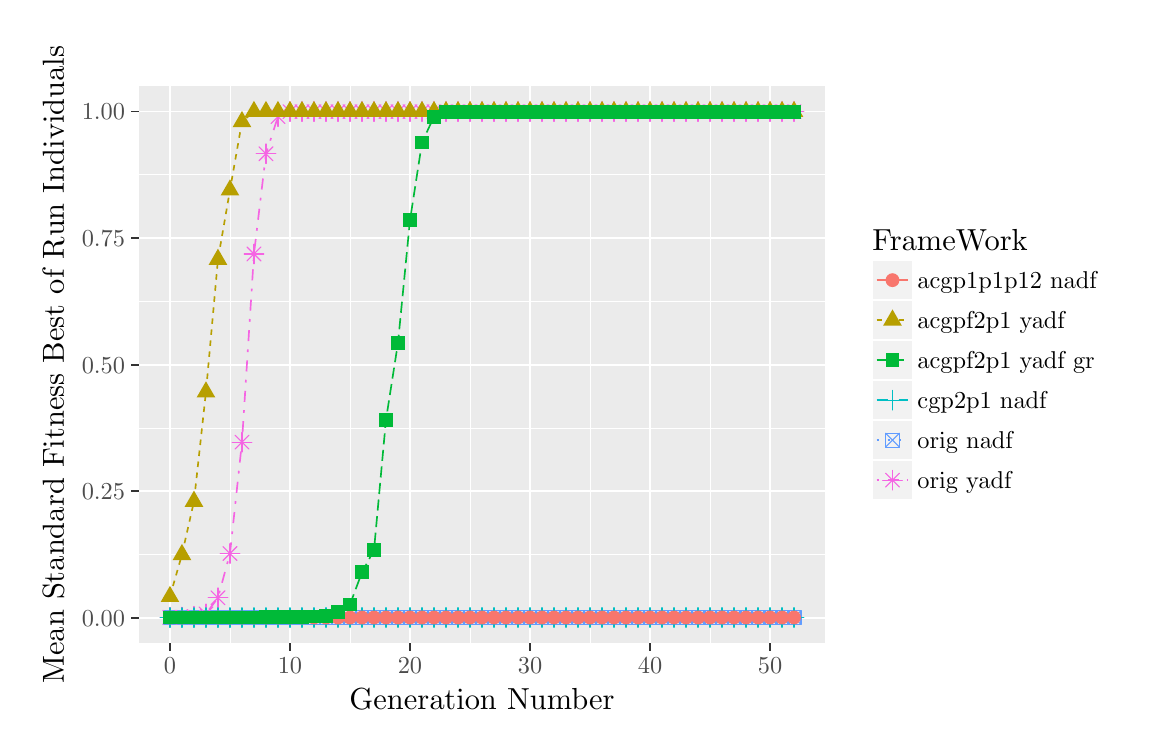
\begin{tikzpicture}[x=1pt,y=1pt]
\definecolor{fillColor}{RGB}{255,255,255}
\path[use as bounding box,fill=fillColor,fill opacity=0.00] (0,0) rectangle (397.48,252.94);
\begin{scope}
\path[clip] (  0.00,  0.00) rectangle (397.48,252.94);
\definecolor{drawColor}{RGB}{255,255,255}
\definecolor{fillColor}{RGB}{255,255,255}

\path[draw=drawColor,line width= 0.6pt,line join=round,line cap=round,fill=fillColor] (  0.00,  0.00) rectangle (397.48,252.95);
\end{scope}
\begin{scope}
\path[clip] ( 40.14, 30.56) rectangle (288.20,231.75);
\definecolor{fillColor}{gray}{0.92}

\path[fill=fillColor] ( 40.14, 30.56) rectangle (288.20,231.75);
\definecolor{drawColor}{RGB}{255,255,255}

\path[draw=drawColor,line width= 0.3pt,line join=round] ( 40.14, 62.57) --
	(288.20, 62.57);

\path[draw=drawColor,line width= 0.3pt,line join=round] ( 40.14,108.29) --
	(288.20,108.29);

\path[draw=drawColor,line width= 0.3pt,line join=round] ( 40.14,154.02) --
	(288.20,154.02);

\path[draw=drawColor,line width= 0.3pt,line join=round] ( 40.14,199.75) --
	(288.20,199.75);

\path[draw=drawColor,line width= 0.3pt,line join=round] ( 73.10, 30.56) --
	( 73.10,231.75);

\path[draw=drawColor,line width= 0.3pt,line join=round] (116.47, 30.56) --
	(116.47,231.75);

\path[draw=drawColor,line width= 0.3pt,line join=round] (159.83, 30.56) --
	(159.83,231.75);

\path[draw=drawColor,line width= 0.3pt,line join=round] (203.20, 30.56) --
	(203.20,231.75);

\path[draw=drawColor,line width= 0.3pt,line join=round] (246.57, 30.56) --
	(246.57,231.75);

\path[draw=drawColor,line width= 0.6pt,line join=round] ( 40.14, 39.70) --
	(288.20, 39.70);

\path[draw=drawColor,line width= 0.6pt,line join=round] ( 40.14, 85.43) --
	(288.20, 85.43);

\path[draw=drawColor,line width= 0.6pt,line join=round] ( 40.14,131.16) --
	(288.20,131.16);

\path[draw=drawColor,line width= 0.6pt,line join=round] ( 40.14,176.88) --
	(288.20,176.88);

\path[draw=drawColor,line width= 0.6pt,line join=round] ( 40.14,222.61) --
	(288.20,222.61);

\path[draw=drawColor,line width= 0.6pt,line join=round] ( 51.41, 30.56) --
	( 51.41,231.75);

\path[draw=drawColor,line width= 0.6pt,line join=round] ( 94.78, 30.56) --
	( 94.78,231.75);

\path[draw=drawColor,line width= 0.6pt,line join=round] (138.15, 30.56) --
	(138.15,231.75);

\path[draw=drawColor,line width= 0.6pt,line join=round] (181.52, 30.56) --
	(181.52,231.75);

\path[draw=drawColor,line width= 0.6pt,line join=round] (224.88, 30.56) --
	(224.88,231.75);

\path[draw=drawColor,line width= 0.6pt,line join=round] (268.25, 30.56) --
	(268.25,231.75);
\definecolor{drawColor}{RGB}{248,118,109}

\path[draw=drawColor,line width= 0.6pt,line join=round] ( 51.41, 39.78) --
	( 55.75, 39.78) --
	( 60.09, 39.78) --
	( 64.42, 39.78) --
	( 68.76, 39.78) --
	( 73.10, 39.78) --
	( 77.43, 39.78) --
	( 81.77, 39.78) --
	( 86.11, 39.78) --
	( 90.44, 39.78) --
	( 94.78, 39.78) --
	( 99.12, 39.78) --
	(103.45, 39.78) --
	(107.79, 39.78) --
	(112.13, 39.79) --
	(116.47, 39.79) --
	(120.80, 39.79) --
	(125.14, 39.79) --
	(129.48, 39.80) --
	(133.81, 39.80) --
	(138.15, 39.80) --
	(142.49, 39.80) --
	(146.82, 39.80) --
	(151.16, 39.80) --
	(155.50, 39.80) --
	(159.83, 39.80) --
	(164.17, 39.80) --
	(168.51, 39.80) --
	(172.84, 39.80) --
	(177.18, 39.80) --
	(181.52, 39.80) --
	(185.85, 39.80) --
	(190.19, 39.80) --
	(194.53, 39.80) --
	(198.86, 39.80) --
	(203.20, 39.80) --
	(207.54, 39.80) --
	(211.87, 39.80) --
	(216.21, 39.80) --
	(220.55, 39.80) --
	(224.88, 39.80) --
	(229.22, 39.80) --
	(233.56, 39.80) --
	(237.89, 39.80) --
	(242.23, 39.80) --
	(246.57, 39.80) --
	(250.90, 39.81) --
	(255.24, 39.81) --
	(259.58, 39.81) --
	(263.91, 39.81) --
	(268.25, 39.81) --
	(272.59, 39.81) --
	(276.92, 39.81);
\definecolor{drawColor}{RGB}{183,159,0}

\path[draw=drawColor,line width= 0.6pt,dash pattern=on 2pt off 2pt ,line join=round] ( 51.41, 47.35) --
	( 55.75, 62.52) --
	( 60.09, 81.76) --
	( 64.42,121.28) --
	( 68.76,169.20) --
	( 73.10,194.26) --
	( 77.43,218.95) --
	( 81.77,222.61) --
	( 86.11,222.61) --
	( 90.44,222.61) --
	( 94.78,222.61) --
	( 99.12,222.61) --
	(103.45,222.61) --
	(107.79,222.61) --
	(112.13,222.61) --
	(116.47,222.61) --
	(120.80,222.61) --
	(125.14,222.61) --
	(129.48,222.61) --
	(133.81,222.61) --
	(138.15,222.61) --
	(142.49,222.61) --
	(146.82,222.61) --
	(151.16,222.61) --
	(155.50,222.61) --
	(159.83,222.61) --
	(164.17,222.61) --
	(168.51,222.61) --
	(172.84,222.61) --
	(177.18,222.61) --
	(181.52,222.61) --
	(185.85,222.61) --
	(190.19,222.61) --
	(194.53,222.61) --
	(198.86,222.61) --
	(203.20,222.61) --
	(207.54,222.61) --
	(211.87,222.61) --
	(216.21,222.61) --
	(220.55,222.61) --
	(224.88,222.61) --
	(229.22,222.61) --
	(233.56,222.61) --
	(237.89,222.61) --
	(242.23,222.61) --
	(246.57,222.61) --
	(250.90,222.61) --
	(255.24,222.61) --
	(259.58,222.61) --
	(263.91,222.61) --
	(268.25,222.61) --
	(272.59,222.61) --
	(276.92,222.61);
\definecolor{drawColor}{RGB}{0,186,56}

\path[draw=drawColor,line width= 0.6pt,dash pattern=on 4pt off 2pt ,line join=round] ( 51.41, 39.78) --
	( 55.75, 39.79) --
	( 60.09, 39.80) --
	( 64.42, 39.80) --
	( 68.76, 39.80) --
	( 73.10, 39.81) --
	( 77.43, 39.82) --
	( 81.77, 39.84) --
	( 86.11, 39.86) --
	( 90.44, 39.88) --
	( 94.78, 39.94) --
	( 99.12, 40.03) --
	(103.45, 40.17) --
	(107.79, 40.38) --
	(112.13, 41.65) --
	(116.47, 44.51) --
	(120.80, 56.14) --
	(125.14, 64.14) --
	(129.48,111.30) --
	(133.81,139.05) --
	(138.15,183.35) --
	(142.49,211.45) --
	(146.82,220.78) --
	(151.16,222.61) --
	(155.50,222.61) --
	(159.83,222.61) --
	(164.17,222.61) --
	(168.51,222.61) --
	(172.84,222.61) --
	(177.18,222.61) --
	(181.52,222.61) --
	(185.85,222.61) --
	(190.19,222.61) --
	(194.53,222.61) --
	(198.86,222.61) --
	(203.20,222.61) --
	(207.54,222.61) --
	(211.87,222.61) --
	(216.21,222.61) --
	(220.55,222.61) --
	(224.88,222.61) --
	(229.22,222.61) --
	(233.56,222.61) --
	(237.89,222.61) --
	(242.23,222.61) --
	(246.57,222.61) --
	(250.90,222.61) --
	(255.24,222.61) --
	(259.58,222.61) --
	(263.91,222.61) --
	(268.25,222.61) --
	(272.59,222.61) --
	(276.92,222.61);
\definecolor{drawColor}{RGB}{0,191,196}

\path[draw=drawColor,line width= 0.6pt,dash pattern=on 4pt off 4pt ,line join=round] ( 51.41, 39.78) --
	( 55.75, 39.78) --
	( 60.09, 39.78) --
	( 64.42, 39.78) --
	( 68.76, 39.78) --
	( 73.10, 39.78) --
	( 77.43, 39.78) --
	( 81.77, 39.78) --
	( 86.11, 39.78) --
	( 90.44, 39.78) --
	( 94.78, 39.78) --
	( 99.12, 39.79) --
	(103.45, 39.79) --
	(107.79, 39.79) --
	(112.13, 39.79) --
	(116.47, 39.80) --
	(120.80, 39.80) --
	(125.14, 39.80) --
	(129.48, 39.80) --
	(133.81, 39.80) --
	(138.15, 39.80) --
	(142.49, 39.80) --
	(146.82, 39.80) --
	(151.16, 39.80) --
	(155.50, 39.80) --
	(159.83, 39.80) --
	(164.17, 39.80) --
	(168.51, 39.80) --
	(172.84, 39.80) --
	(177.18, 39.80) --
	(181.52, 39.80) --
	(185.85, 39.80) --
	(190.19, 39.80) --
	(194.53, 39.80) --
	(198.86, 39.80) --
	(203.20, 39.80) --
	(207.54, 39.80) --
	(211.87, 39.80) --
	(216.21, 39.80) --
	(220.55, 39.80) --
	(224.88, 39.80) --
	(229.22, 39.81) --
	(233.56, 39.81) --
	(237.89, 39.81) --
	(242.23, 39.81) --
	(246.57, 39.81) --
	(250.90, 39.81) --
	(255.24, 39.81) --
	(259.58, 39.81) --
	(263.91, 39.81) --
	(268.25, 39.81) --
	(272.59, 39.81) --
	(276.92, 39.81);
\definecolor{drawColor}{RGB}{97,156,255}

\path[draw=drawColor,line width= 0.6pt,dash pattern=on 1pt off 3pt ,line join=round] ( 51.41, 39.78) --
	( 55.75, 39.78) --
	( 60.09, 39.78) --
	( 64.42, 39.78) --
	( 68.76, 39.78) --
	( 73.10, 39.78) --
	( 77.43, 39.78) --
	( 81.77, 39.78) --
	( 86.11, 39.78) --
	( 90.44, 39.78) --
	( 94.78, 39.78) --
	( 99.12, 39.78) --
	(103.45, 39.78) --
	(107.79, 39.78) --
	(112.13, 39.78) --
	(116.47, 39.79) --
	(120.80, 39.79) --
	(125.14, 39.79) --
	(129.48, 39.79) --
	(133.81, 39.79) --
	(138.15, 39.80) --
	(142.49, 39.80) --
	(146.82, 39.80) --
	(151.16, 39.80) --
	(155.50, 39.80) --
	(159.83, 39.80) --
	(164.17, 39.80) --
	(168.51, 39.80) --
	(172.84, 39.80) --
	(177.18, 39.80) --
	(181.52, 39.80) --
	(185.85, 39.80) --
	(190.19, 39.80) --
	(194.53, 39.80) --
	(198.86, 39.80) --
	(203.20, 39.80) --
	(207.54, 39.80) --
	(211.87, 39.80) --
	(216.21, 39.80) --
	(220.55, 39.80) --
	(224.88, 39.80) --
	(229.22, 39.80) --
	(233.56, 39.80) --
	(237.89, 39.80) --
	(242.23, 39.80) --
	(246.57, 39.80) --
	(250.90, 39.80) --
	(255.24, 39.80) --
	(259.58, 39.80) --
	(263.91, 39.80) --
	(268.25, 39.81) --
	(272.59, 39.81) --
	(276.92, 39.81);
\definecolor{drawColor}{RGB}{245,100,227}

\path[draw=drawColor,line width= 0.6pt,dash pattern=on 1pt off 3pt on 4pt off 3pt ,line join=round] ( 51.41, 39.88) --
	( 55.75, 39.96) --
	( 60.09, 40.23) --
	( 64.42, 41.12) --
	( 68.76, 46.94) --
	( 73.10, 62.93) --
	( 77.43,103.15) --
	( 81.77,171.16) --
	( 86.11,207.37) --
	( 90.44,220.78) --
	( 94.78,222.61) --
	( 99.12,222.61) --
	(103.45,222.61) --
	(107.79,222.61) --
	(112.13,222.61) --
	(116.47,222.61) --
	(120.80,222.61) --
	(125.14,222.61) --
	(129.48,222.61) --
	(133.81,222.61) --
	(138.15,222.61) --
	(142.49,222.61) --
	(146.82,222.61) --
	(151.16,222.61) --
	(155.50,222.61) --
	(159.83,222.61) --
	(164.17,222.61) --
	(168.51,222.61) --
	(172.84,222.61) --
	(177.18,222.61) --
	(181.52,222.61) --
	(185.85,222.61) --
	(190.19,222.61) --
	(194.53,222.61) --
	(198.86,222.61) --
	(203.20,222.61) --
	(207.54,222.61) --
	(211.87,222.61) --
	(216.21,222.61) --
	(220.55,222.61) --
	(224.88,222.61) --
	(229.22,222.61) --
	(233.56,222.61) --
	(237.89,222.61) --
	(242.23,222.61) --
	(246.57,222.61) --
	(250.90,222.61) --
	(255.24,222.61) --
	(259.58,222.61) --
	(263.91,222.61) --
	(268.25,222.61) --
	(272.59,222.61) --
	(276.92,222.61);
\definecolor{drawColor}{RGB}{97,156,255}

\path[draw=drawColor,line width= 0.4pt,line join=round,line cap=round] ( 48.92, 37.28) rectangle ( 53.91, 42.27);

\path[draw=drawColor,line width= 0.4pt,line join=round,line cap=round] ( 48.92, 37.28) -- ( 53.91, 42.27);

\path[draw=drawColor,line width= 0.4pt,line join=round,line cap=round] ( 48.92, 42.27) -- ( 53.91, 37.28);

\path[draw=drawColor,line width= 0.4pt,line join=round,line cap=round] ( 53.25, 37.28) rectangle ( 58.25, 42.27);

\path[draw=drawColor,line width= 0.4pt,line join=round,line cap=round] ( 53.25, 37.28) -- ( 58.25, 42.27);

\path[draw=drawColor,line width= 0.4pt,line join=round,line cap=round] ( 53.25, 42.27) -- ( 58.25, 37.28);

\path[draw=drawColor,line width= 0.4pt,line join=round,line cap=round] ( 57.59, 37.28) rectangle ( 62.59, 42.27);

\path[draw=drawColor,line width= 0.4pt,line join=round,line cap=round] ( 57.59, 37.28) -- ( 62.59, 42.27);

\path[draw=drawColor,line width= 0.4pt,line join=round,line cap=round] ( 57.59, 42.27) -- ( 62.59, 37.28);

\path[draw=drawColor,line width= 0.4pt,line join=round,line cap=round] ( 61.93, 37.28) rectangle ( 66.92, 42.27);

\path[draw=drawColor,line width= 0.4pt,line join=round,line cap=round] ( 61.93, 37.28) -- ( 66.92, 42.27);

\path[draw=drawColor,line width= 0.4pt,line join=round,line cap=round] ( 61.93, 42.27) -- ( 66.92, 37.28);

\path[draw=drawColor,line width= 0.4pt,line join=round,line cap=round] ( 66.26, 37.28) rectangle ( 71.26, 42.27);

\path[draw=drawColor,line width= 0.4pt,line join=round,line cap=round] ( 66.26, 37.28) -- ( 71.26, 42.27);

\path[draw=drawColor,line width= 0.4pt,line join=round,line cap=round] ( 66.26, 42.27) -- ( 71.26, 37.28);

\path[draw=drawColor,line width= 0.4pt,line join=round,line cap=round] ( 70.60, 37.28) rectangle ( 75.60, 42.27);

\path[draw=drawColor,line width= 0.4pt,line join=round,line cap=round] ( 70.60, 37.28) -- ( 75.60, 42.27);

\path[draw=drawColor,line width= 0.4pt,line join=round,line cap=round] ( 70.60, 42.27) -- ( 75.60, 37.28);

\path[draw=drawColor,line width= 0.4pt,line join=round,line cap=round] ( 74.94, 37.28) rectangle ( 79.93, 42.27);

\path[draw=drawColor,line width= 0.4pt,line join=round,line cap=round] ( 74.94, 37.28) -- ( 79.93, 42.27);

\path[draw=drawColor,line width= 0.4pt,line join=round,line cap=round] ( 74.94, 42.27) -- ( 79.93, 37.28);

\path[draw=drawColor,line width= 0.4pt,line join=round,line cap=round] ( 79.27, 37.28) rectangle ( 84.27, 42.27);

\path[draw=drawColor,line width= 0.4pt,line join=round,line cap=round] ( 79.27, 37.28) -- ( 84.27, 42.27);

\path[draw=drawColor,line width= 0.4pt,line join=round,line cap=round] ( 79.27, 42.27) -- ( 84.27, 37.28);

\path[draw=drawColor,line width= 0.4pt,line join=round,line cap=round] ( 83.61, 37.28) rectangle ( 88.61, 42.27);

\path[draw=drawColor,line width= 0.4pt,line join=round,line cap=round] ( 83.61, 37.28) -- ( 88.61, 42.27);

\path[draw=drawColor,line width= 0.4pt,line join=round,line cap=round] ( 83.61, 42.27) -- ( 88.61, 37.28);

\path[draw=drawColor,line width= 0.4pt,line join=round,line cap=round] ( 87.95, 37.28) rectangle ( 92.94, 42.27);

\path[draw=drawColor,line width= 0.4pt,line join=round,line cap=round] ( 87.95, 37.28) -- ( 92.94, 42.27);

\path[draw=drawColor,line width= 0.4pt,line join=round,line cap=round] ( 87.95, 42.27) -- ( 92.94, 37.28);

\path[draw=drawColor,line width= 0.4pt,line join=round,line cap=round] ( 92.28, 37.28) rectangle ( 97.28, 42.27);

\path[draw=drawColor,line width= 0.4pt,line join=round,line cap=round] ( 92.28, 37.28) -- ( 97.28, 42.27);

\path[draw=drawColor,line width= 0.4pt,line join=round,line cap=round] ( 92.28, 42.27) -- ( 97.28, 37.28);

\path[draw=drawColor,line width= 0.4pt,line join=round,line cap=round] ( 96.62, 37.28) rectangle (101.62, 42.28);

\path[draw=drawColor,line width= 0.4pt,line join=round,line cap=round] ( 96.62, 37.28) -- (101.62, 42.28);

\path[draw=drawColor,line width= 0.4pt,line join=round,line cap=round] ( 96.62, 42.28) -- (101.62, 37.28);

\path[draw=drawColor,line width= 0.4pt,line join=round,line cap=round] (100.96, 37.28) rectangle (105.95, 42.28);

\path[draw=drawColor,line width= 0.4pt,line join=round,line cap=round] (100.96, 37.28) -- (105.95, 42.28);

\path[draw=drawColor,line width= 0.4pt,line join=round,line cap=round] (100.96, 42.28) -- (105.95, 37.28);

\path[draw=drawColor,line width= 0.4pt,line join=round,line cap=round] (105.29, 37.28) rectangle (110.29, 42.28);

\path[draw=drawColor,line width= 0.4pt,line join=round,line cap=round] (105.29, 37.28) -- (110.29, 42.28);

\path[draw=drawColor,line width= 0.4pt,line join=round,line cap=round] (105.29, 42.28) -- (110.29, 37.28);

\path[draw=drawColor,line width= 0.4pt,line join=round,line cap=round] (109.63, 37.28) rectangle (114.63, 42.28);

\path[draw=drawColor,line width= 0.4pt,line join=round,line cap=round] (109.63, 37.28) -- (114.63, 42.28);

\path[draw=drawColor,line width= 0.4pt,line join=round,line cap=round] (109.63, 42.28) -- (114.63, 37.28);

\path[draw=drawColor,line width= 0.4pt,line join=round,line cap=round] (113.97, 37.29) rectangle (118.96, 42.28);

\path[draw=drawColor,line width= 0.4pt,line join=round,line cap=round] (113.97, 37.29) -- (118.96, 42.28);

\path[draw=drawColor,line width= 0.4pt,line join=round,line cap=round] (113.97, 42.28) -- (118.96, 37.29);

\path[draw=drawColor,line width= 0.4pt,line join=round,line cap=round] (118.30, 37.29) rectangle (123.30, 42.29);

\path[draw=drawColor,line width= 0.4pt,line join=round,line cap=round] (118.30, 37.29) -- (123.30, 42.29);

\path[draw=drawColor,line width= 0.4pt,line join=round,line cap=round] (118.30, 42.29) -- (123.30, 37.29);

\path[draw=drawColor,line width= 0.4pt,line join=round,line cap=round] (122.64, 37.30) rectangle (127.64, 42.29);

\path[draw=drawColor,line width= 0.4pt,line join=round,line cap=round] (122.64, 37.30) -- (127.64, 42.29);

\path[draw=drawColor,line width= 0.4pt,line join=round,line cap=round] (122.64, 42.29) -- (127.64, 37.30);

\path[draw=drawColor,line width= 0.4pt,line join=round,line cap=round] (126.98, 37.30) rectangle (131.97, 42.29);

\path[draw=drawColor,line width= 0.4pt,line join=round,line cap=round] (126.98, 37.30) -- (131.97, 42.29);

\path[draw=drawColor,line width= 0.4pt,line join=round,line cap=round] (126.98, 42.29) -- (131.97, 37.30);

\path[draw=drawColor,line width= 0.4pt,line join=round,line cap=round] (131.31, 37.30) rectangle (136.31, 42.29);

\path[draw=drawColor,line width= 0.4pt,line join=round,line cap=round] (131.31, 37.30) -- (136.31, 42.29);

\path[draw=drawColor,line width= 0.4pt,line join=round,line cap=round] (131.31, 42.29) -- (136.31, 37.30);

\path[draw=drawColor,line width= 0.4pt,line join=round,line cap=round] (135.65, 37.30) rectangle (140.65, 42.29);

\path[draw=drawColor,line width= 0.4pt,line join=round,line cap=round] (135.65, 37.30) -- (140.65, 42.29);

\path[draw=drawColor,line width= 0.4pt,line join=round,line cap=round] (135.65, 42.29) -- (140.65, 37.30);

\path[draw=drawColor,line width= 0.4pt,line join=round,line cap=round] (139.99, 37.30) rectangle (144.98, 42.29);

\path[draw=drawColor,line width= 0.4pt,line join=round,line cap=round] (139.99, 37.30) -- (144.98, 42.29);

\path[draw=drawColor,line width= 0.4pt,line join=round,line cap=round] (139.99, 42.29) -- (144.98, 37.30);

\path[draw=drawColor,line width= 0.4pt,line join=round,line cap=round] (144.32, 37.30) rectangle (149.32, 42.29);

\path[draw=drawColor,line width= 0.4pt,line join=round,line cap=round] (144.32, 37.30) -- (149.32, 42.29);

\path[draw=drawColor,line width= 0.4pt,line join=round,line cap=round] (144.32, 42.29) -- (149.32, 37.30);

\path[draw=drawColor,line width= 0.4pt,line join=round,line cap=round] (148.66, 37.30) rectangle (153.66, 42.29);

\path[draw=drawColor,line width= 0.4pt,line join=round,line cap=round] (148.66, 37.30) -- (153.66, 42.29);

\path[draw=drawColor,line width= 0.4pt,line join=round,line cap=round] (148.66, 42.29) -- (153.66, 37.30);

\path[draw=drawColor,line width= 0.4pt,line join=round,line cap=round] (153.00, 37.30) rectangle (157.99, 42.29);

\path[draw=drawColor,line width= 0.4pt,line join=round,line cap=round] (153.00, 37.30) -- (157.99, 42.29);

\path[draw=drawColor,line width= 0.4pt,line join=round,line cap=round] (153.00, 42.29) -- (157.99, 37.30);

\path[draw=drawColor,line width= 0.4pt,line join=round,line cap=round] (157.33, 37.30) rectangle (162.33, 42.29);

\path[draw=drawColor,line width= 0.4pt,line join=round,line cap=round] (157.33, 37.30) -- (162.33, 42.29);

\path[draw=drawColor,line width= 0.4pt,line join=round,line cap=round] (157.33, 42.29) -- (162.33, 37.30);

\path[draw=drawColor,line width= 0.4pt,line join=round,line cap=round] (161.67, 37.30) rectangle (166.67, 42.29);

\path[draw=drawColor,line width= 0.4pt,line join=round,line cap=round] (161.67, 37.30) -- (166.67, 42.29);

\path[draw=drawColor,line width= 0.4pt,line join=round,line cap=round] (161.67, 42.29) -- (166.67, 37.30);

\path[draw=drawColor,line width= 0.4pt,line join=round,line cap=round] (166.01, 37.30) rectangle (171.00, 42.29);

\path[draw=drawColor,line width= 0.4pt,line join=round,line cap=round] (166.01, 37.30) -- (171.00, 42.29);

\path[draw=drawColor,line width= 0.4pt,line join=round,line cap=round] (166.01, 42.29) -- (171.00, 37.30);

\path[draw=drawColor,line width= 0.4pt,line join=round,line cap=round] (170.35, 37.30) rectangle (175.34, 42.29);

\path[draw=drawColor,line width= 0.4pt,line join=round,line cap=round] (170.35, 37.30) -- (175.34, 42.29);

\path[draw=drawColor,line width= 0.4pt,line join=round,line cap=round] (170.35, 42.29) -- (175.34, 37.30);

\path[draw=drawColor,line width= 0.4pt,line join=round,line cap=round] (174.68, 37.30) rectangle (179.68, 42.29);

\path[draw=drawColor,line width= 0.4pt,line join=round,line cap=round] (174.68, 37.30) -- (179.68, 42.29);

\path[draw=drawColor,line width= 0.4pt,line join=round,line cap=round] (174.68, 42.29) -- (179.68, 37.30);

\path[draw=drawColor,line width= 0.4pt,line join=round,line cap=round] (179.02, 37.30) rectangle (184.01, 42.29);

\path[draw=drawColor,line width= 0.4pt,line join=round,line cap=round] (179.02, 37.30) -- (184.01, 42.29);

\path[draw=drawColor,line width= 0.4pt,line join=round,line cap=round] (179.02, 42.29) -- (184.01, 37.30);

\path[draw=drawColor,line width= 0.4pt,line join=round,line cap=round] (183.36, 37.30) rectangle (188.35, 42.29);

\path[draw=drawColor,line width= 0.4pt,line join=round,line cap=round] (183.36, 37.30) -- (188.35, 42.29);

\path[draw=drawColor,line width= 0.4pt,line join=round,line cap=round] (183.36, 42.29) -- (188.35, 37.30);

\path[draw=drawColor,line width= 0.4pt,line join=round,line cap=round] (187.69, 37.30) rectangle (192.69, 42.29);

\path[draw=drawColor,line width= 0.4pt,line join=round,line cap=round] (187.69, 37.30) -- (192.69, 42.29);

\path[draw=drawColor,line width= 0.4pt,line join=round,line cap=round] (187.69, 42.29) -- (192.69, 37.30);

\path[draw=drawColor,line width= 0.4pt,line join=round,line cap=round] (192.03, 37.30) rectangle (197.02, 42.29);

\path[draw=drawColor,line width= 0.4pt,line join=round,line cap=round] (192.03, 37.30) -- (197.02, 42.29);

\path[draw=drawColor,line width= 0.4pt,line join=round,line cap=round] (192.03, 42.29) -- (197.02, 37.30);

\path[draw=drawColor,line width= 0.4pt,line join=round,line cap=round] (196.37, 37.30) rectangle (201.36, 42.29);

\path[draw=drawColor,line width= 0.4pt,line join=round,line cap=round] (196.37, 37.30) -- (201.36, 42.29);

\path[draw=drawColor,line width= 0.4pt,line join=round,line cap=round] (196.37, 42.29) -- (201.36, 37.30);

\path[draw=drawColor,line width= 0.4pt,line join=round,line cap=round] (200.70, 37.30) rectangle (205.70, 42.29);

\path[draw=drawColor,line width= 0.4pt,line join=round,line cap=round] (200.70, 37.30) -- (205.70, 42.29);

\path[draw=drawColor,line width= 0.4pt,line join=round,line cap=round] (200.70, 42.29) -- (205.70, 37.30);

\path[draw=drawColor,line width= 0.4pt,line join=round,line cap=round] (205.04, 37.30) rectangle (210.03, 42.29);

\path[draw=drawColor,line width= 0.4pt,line join=round,line cap=round] (205.04, 37.30) -- (210.03, 42.29);

\path[draw=drawColor,line width= 0.4pt,line join=round,line cap=round] (205.04, 42.29) -- (210.03, 37.30);

\path[draw=drawColor,line width= 0.4pt,line join=round,line cap=round] (209.38, 37.30) rectangle (214.37, 42.29);

\path[draw=drawColor,line width= 0.4pt,line join=round,line cap=round] (209.38, 37.30) -- (214.37, 42.29);

\path[draw=drawColor,line width= 0.4pt,line join=round,line cap=round] (209.38, 42.29) -- (214.37, 37.30);

\path[draw=drawColor,line width= 0.4pt,line join=round,line cap=round] (213.71, 37.30) rectangle (218.71, 42.29);

\path[draw=drawColor,line width= 0.4pt,line join=round,line cap=round] (213.71, 37.30) -- (218.71, 42.29);

\path[draw=drawColor,line width= 0.4pt,line join=round,line cap=round] (213.71, 42.29) -- (218.71, 37.30);

\path[draw=drawColor,line width= 0.4pt,line join=round,line cap=round] (218.05, 37.30) rectangle (223.04, 42.29);

\path[draw=drawColor,line width= 0.4pt,line join=round,line cap=round] (218.05, 37.30) -- (223.04, 42.29);

\path[draw=drawColor,line width= 0.4pt,line join=round,line cap=round] (218.05, 42.29) -- (223.04, 37.30);

\path[draw=drawColor,line width= 0.4pt,line join=round,line cap=round] (222.39, 37.30) rectangle (227.38, 42.30);

\path[draw=drawColor,line width= 0.4pt,line join=round,line cap=round] (222.39, 37.30) -- (227.38, 42.30);

\path[draw=drawColor,line width= 0.4pt,line join=round,line cap=round] (222.39, 42.30) -- (227.38, 37.30);

\path[draw=drawColor,line width= 0.4pt,line join=round,line cap=round] (226.72, 37.30) rectangle (231.72, 42.30);

\path[draw=drawColor,line width= 0.4pt,line join=round,line cap=round] (226.72, 37.30) -- (231.72, 42.30);

\path[draw=drawColor,line width= 0.4pt,line join=round,line cap=round] (226.72, 42.30) -- (231.72, 37.30);

\path[draw=drawColor,line width= 0.4pt,line join=round,line cap=round] (231.06, 37.30) rectangle (236.05, 42.30);

\path[draw=drawColor,line width= 0.4pt,line join=round,line cap=round] (231.06, 37.30) -- (236.05, 42.30);

\path[draw=drawColor,line width= 0.4pt,line join=round,line cap=round] (231.06, 42.30) -- (236.05, 37.30);

\path[draw=drawColor,line width= 0.4pt,line join=round,line cap=round] (235.40, 37.30) rectangle (240.39, 42.30);

\path[draw=drawColor,line width= 0.4pt,line join=round,line cap=round] (235.40, 37.30) -- (240.39, 42.30);

\path[draw=drawColor,line width= 0.4pt,line join=round,line cap=round] (235.40, 42.30) -- (240.39, 37.30);

\path[draw=drawColor,line width= 0.4pt,line join=round,line cap=round] (239.73, 37.30) rectangle (244.73, 42.30);

\path[draw=drawColor,line width= 0.4pt,line join=round,line cap=round] (239.73, 37.30) -- (244.73, 42.30);

\path[draw=drawColor,line width= 0.4pt,line join=round,line cap=round] (239.73, 42.30) -- (244.73, 37.30);

\path[draw=drawColor,line width= 0.4pt,line join=round,line cap=round] (244.07, 37.30) rectangle (249.06, 42.30);

\path[draw=drawColor,line width= 0.4pt,line join=round,line cap=round] (244.07, 37.30) -- (249.06, 42.30);

\path[draw=drawColor,line width= 0.4pt,line join=round,line cap=round] (244.07, 42.30) -- (249.06, 37.30);

\path[draw=drawColor,line width= 0.4pt,line join=round,line cap=round] (248.41, 37.30) rectangle (253.40, 42.30);

\path[draw=drawColor,line width= 0.4pt,line join=round,line cap=round] (248.41, 37.30) -- (253.40, 42.30);

\path[draw=drawColor,line width= 0.4pt,line join=round,line cap=round] (248.41, 42.30) -- (253.40, 37.30);

\path[draw=drawColor,line width= 0.4pt,line join=round,line cap=round] (252.74, 37.30) rectangle (257.74, 42.30);

\path[draw=drawColor,line width= 0.4pt,line join=round,line cap=round] (252.74, 37.30) -- (257.74, 42.30);

\path[draw=drawColor,line width= 0.4pt,line join=round,line cap=round] (252.74, 42.30) -- (257.74, 37.30);

\path[draw=drawColor,line width= 0.4pt,line join=round,line cap=round] (257.08, 37.31) rectangle (262.07, 42.30);

\path[draw=drawColor,line width= 0.4pt,line join=round,line cap=round] (257.08, 37.31) -- (262.07, 42.30);

\path[draw=drawColor,line width= 0.4pt,line join=round,line cap=round] (257.08, 42.30) -- (262.07, 37.31);

\path[draw=drawColor,line width= 0.4pt,line join=round,line cap=round] (261.42, 37.31) rectangle (266.41, 42.30);

\path[draw=drawColor,line width= 0.4pt,line join=round,line cap=round] (261.42, 37.31) -- (266.41, 42.30);

\path[draw=drawColor,line width= 0.4pt,line join=round,line cap=round] (261.42, 42.30) -- (266.41, 37.31);

\path[draw=drawColor,line width= 0.4pt,line join=round,line cap=round] (265.75, 37.31) rectangle (270.75, 42.30);

\path[draw=drawColor,line width= 0.4pt,line join=round,line cap=round] (265.75, 37.31) -- (270.75, 42.30);

\path[draw=drawColor,line width= 0.4pt,line join=round,line cap=round] (265.75, 42.30) -- (270.75, 37.31);

\path[draw=drawColor,line width= 0.4pt,line join=round,line cap=round] (270.09, 37.31) rectangle (275.09, 42.30);

\path[draw=drawColor,line width= 0.4pt,line join=round,line cap=round] (270.09, 37.31) -- (275.09, 42.30);

\path[draw=drawColor,line width= 0.4pt,line join=round,line cap=round] (270.09, 42.30) -- (275.09, 37.31);

\path[draw=drawColor,line width= 0.4pt,line join=round,line cap=round] (274.43, 37.31) rectangle (279.42, 42.30);

\path[draw=drawColor,line width= 0.4pt,line join=round,line cap=round] (274.43, 37.31) -- (279.42, 42.30);

\path[draw=drawColor,line width= 0.4pt,line join=round,line cap=round] (274.43, 42.30) -- (279.42, 37.31);
\definecolor{drawColor}{RGB}{245,100,227}

\path[draw=drawColor,line width= 0.4pt,line join=round,line cap=round] ( 48.92, 37.39) -- ( 53.91, 42.38);

\path[draw=drawColor,line width= 0.4pt,line join=round,line cap=round] ( 48.92, 42.38) -- ( 53.91, 37.39);

\path[draw=drawColor,line width= 0.4pt,line join=round,line cap=round] ( 47.88, 39.88) -- ( 54.95, 39.88);

\path[draw=drawColor,line width= 0.4pt,line join=round,line cap=round] ( 51.41, 36.35) -- ( 51.41, 43.42);

\path[draw=drawColor,line width= 0.4pt,line join=round,line cap=round] ( 53.25, 37.46) -- ( 58.25, 42.46);

\path[draw=drawColor,line width= 0.4pt,line join=round,line cap=round] ( 53.25, 42.46) -- ( 58.25, 37.46);

\path[draw=drawColor,line width= 0.4pt,line join=round,line cap=round] ( 52.22, 39.96) -- ( 59.28, 39.96);

\path[draw=drawColor,line width= 0.4pt,line join=round,line cap=round] ( 55.75, 36.43) -- ( 55.75, 43.49);

\path[draw=drawColor,line width= 0.4pt,line join=round,line cap=round] ( 57.59, 37.74) -- ( 62.59, 42.73);

\path[draw=drawColor,line width= 0.4pt,line join=round,line cap=round] ( 57.59, 42.73) -- ( 62.59, 37.74);

\path[draw=drawColor,line width= 0.4pt,line join=round,line cap=round] ( 56.56, 40.23) -- ( 63.62, 40.23);

\path[draw=drawColor,line width= 0.4pt,line join=round,line cap=round] ( 60.09, 36.70) -- ( 60.09, 43.77);

\path[draw=drawColor,line width= 0.4pt,line join=round,line cap=round] ( 61.93, 38.62) -- ( 66.92, 43.62);

\path[draw=drawColor,line width= 0.4pt,line join=round,line cap=round] ( 61.93, 43.62) -- ( 66.92, 38.62);

\path[draw=drawColor,line width= 0.4pt,line join=round,line cap=round] ( 60.89, 41.12) -- ( 67.96, 41.12);

\path[draw=drawColor,line width= 0.4pt,line join=round,line cap=round] ( 64.42, 37.59) -- ( 64.42, 44.65);

\path[draw=drawColor,line width= 0.4pt,line join=round,line cap=round] ( 66.26, 44.44) -- ( 71.26, 49.44);

\path[draw=drawColor,line width= 0.4pt,line join=round,line cap=round] ( 66.26, 49.44) -- ( 71.26, 44.44);

\path[draw=drawColor,line width= 0.4pt,line join=round,line cap=round] ( 65.23, 46.94) -- ( 72.29, 46.94);

\path[draw=drawColor,line width= 0.4pt,line join=round,line cap=round] ( 68.76, 43.41) -- ( 68.76, 50.47);

\path[draw=drawColor,line width= 0.4pt,line join=round,line cap=round] ( 70.60, 60.43) -- ( 75.60, 65.42);

\path[draw=drawColor,line width= 0.4pt,line join=round,line cap=round] ( 70.60, 65.42) -- ( 75.60, 60.43);

\path[draw=drawColor,line width= 0.4pt,line join=round,line cap=round] ( 69.57, 62.93) -- ( 76.63, 62.93);

\path[draw=drawColor,line width= 0.4pt,line join=round,line cap=round] ( 73.10, 59.40) -- ( 73.10, 66.46);

\path[draw=drawColor,line width= 0.4pt,line join=round,line cap=round] ( 74.94,100.66) -- ( 79.93,105.65);

\path[draw=drawColor,line width= 0.4pt,line join=round,line cap=round] ( 74.94,105.65) -- ( 79.93,100.66);

\path[draw=drawColor,line width= 0.4pt,line join=round,line cap=round] ( 73.90,103.15) -- ( 80.97,103.15);

\path[draw=drawColor,line width= 0.4pt,line join=round,line cap=round] ( 77.43, 99.62) -- ( 77.43,106.69);

\path[draw=drawColor,line width= 0.4pt,line join=round,line cap=round] ( 79.27,168.66) -- ( 84.27,173.66);

\path[draw=drawColor,line width= 0.4pt,line join=round,line cap=round] ( 79.27,173.66) -- ( 84.27,168.66);

\path[draw=drawColor,line width= 0.4pt,line join=round,line cap=round] ( 78.24,171.16) -- ( 85.30,171.16);

\path[draw=drawColor,line width= 0.4pt,line join=round,line cap=round] ( 81.77,167.63) -- ( 81.77,174.69);

\path[draw=drawColor,line width= 0.4pt,line join=round,line cap=round] ( 83.61,204.87) -- ( 88.61,209.86);

\path[draw=drawColor,line width= 0.4pt,line join=round,line cap=round] ( 83.61,209.86) -- ( 88.61,204.87);

\path[draw=drawColor,line width= 0.4pt,line join=round,line cap=round] ( 82.58,207.37) -- ( 89.64,207.37);

\path[draw=drawColor,line width= 0.4pt,line join=round,line cap=round] ( 86.11,203.83) -- ( 86.11,210.90);

\path[draw=drawColor,line width= 0.4pt,line join=round,line cap=round] ( 87.95,218.28) -- ( 92.94,223.28);

\path[draw=drawColor,line width= 0.4pt,line join=round,line cap=round] ( 87.95,223.28) -- ( 92.94,218.28);

\path[draw=drawColor,line width= 0.4pt,line join=round,line cap=round] ( 86.91,220.78) -- ( 93.98,220.78);

\path[draw=drawColor,line width= 0.4pt,line join=round,line cap=round] ( 90.44,217.25) -- ( 90.44,224.31);

\path[draw=drawColor,line width= 0.4pt,line join=round,line cap=round] ( 92.28,220.11) -- ( 97.28,225.11);

\path[draw=drawColor,line width= 0.4pt,line join=round,line cap=round] ( 92.28,225.11) -- ( 97.28,220.11);

\path[draw=drawColor,line width= 0.4pt,line join=round,line cap=round] ( 91.25,222.61) -- ( 98.31,222.61);

\path[draw=drawColor,line width= 0.4pt,line join=round,line cap=round] ( 94.78,219.08) -- ( 94.78,226.14);

\path[draw=drawColor,line width= 0.4pt,line join=round,line cap=round] ( 96.62,220.11) -- (101.62,225.11);

\path[draw=drawColor,line width= 0.4pt,line join=round,line cap=round] ( 96.62,225.11) -- (101.62,220.11);

\path[draw=drawColor,line width= 0.4pt,line join=round,line cap=round] ( 95.59,222.61) -- (102.65,222.61);

\path[draw=drawColor,line width= 0.4pt,line join=round,line cap=round] ( 99.12,219.08) -- ( 99.12,226.14);

\path[draw=drawColor,line width= 0.4pt,line join=round,line cap=round] (100.96,220.11) -- (105.95,225.11);

\path[draw=drawColor,line width= 0.4pt,line join=round,line cap=round] (100.96,225.11) -- (105.95,220.11);

\path[draw=drawColor,line width= 0.4pt,line join=round,line cap=round] ( 99.92,222.61) -- (106.99,222.61);

\path[draw=drawColor,line width= 0.4pt,line join=round,line cap=round] (103.45,219.08) -- (103.45,226.14);

\path[draw=drawColor,line width= 0.4pt,line join=round,line cap=round] (105.29,220.11) -- (110.29,225.11);

\path[draw=drawColor,line width= 0.4pt,line join=round,line cap=round] (105.29,225.11) -- (110.29,220.11);

\path[draw=drawColor,line width= 0.4pt,line join=round,line cap=round] (104.26,222.61) -- (111.32,222.61);

\path[draw=drawColor,line width= 0.4pt,line join=round,line cap=round] (107.79,219.08) -- (107.79,226.14);

\path[draw=drawColor,line width= 0.4pt,line join=round,line cap=round] (109.63,220.11) -- (114.63,225.11);

\path[draw=drawColor,line width= 0.4pt,line join=round,line cap=round] (109.63,225.11) -- (114.63,220.11);

\path[draw=drawColor,line width= 0.4pt,line join=round,line cap=round] (108.60,222.61) -- (115.66,222.61);

\path[draw=drawColor,line width= 0.4pt,line join=round,line cap=round] (112.13,219.08) -- (112.13,226.14);

\path[draw=drawColor,line width= 0.4pt,line join=round,line cap=round] (113.97,220.11) -- (118.96,225.11);

\path[draw=drawColor,line width= 0.4pt,line join=round,line cap=round] (113.97,225.11) -- (118.96,220.11);

\path[draw=drawColor,line width= 0.4pt,line join=round,line cap=round] (112.93,222.61) -- (120.00,222.61);

\path[draw=drawColor,line width= 0.4pt,line join=round,line cap=round] (116.47,219.08) -- (116.47,226.14);

\path[draw=drawColor,line width= 0.4pt,line join=round,line cap=round] (118.30,220.11) -- (123.30,225.11);

\path[draw=drawColor,line width= 0.4pt,line join=round,line cap=round] (118.30,225.11) -- (123.30,220.11);

\path[draw=drawColor,line width= 0.4pt,line join=round,line cap=round] (117.27,222.61) -- (124.33,222.61);

\path[draw=drawColor,line width= 0.4pt,line join=round,line cap=round] (120.80,219.08) -- (120.80,226.14);

\path[draw=drawColor,line width= 0.4pt,line join=round,line cap=round] (122.64,220.11) -- (127.64,225.11);

\path[draw=drawColor,line width= 0.4pt,line join=round,line cap=round] (122.64,225.11) -- (127.64,220.11);

\path[draw=drawColor,line width= 0.4pt,line join=round,line cap=round] (121.61,222.61) -- (128.67,222.61);

\path[draw=drawColor,line width= 0.4pt,line join=round,line cap=round] (125.14,219.08) -- (125.14,226.14);

\path[draw=drawColor,line width= 0.4pt,line join=round,line cap=round] (126.98,220.11) -- (131.97,225.11);

\path[draw=drawColor,line width= 0.4pt,line join=round,line cap=round] (126.98,225.11) -- (131.97,220.11);

\path[draw=drawColor,line width= 0.4pt,line join=round,line cap=round] (125.94,222.61) -- (133.01,222.61);

\path[draw=drawColor,line width= 0.4pt,line join=round,line cap=round] (129.48,219.08) -- (129.48,226.14);

\path[draw=drawColor,line width= 0.4pt,line join=round,line cap=round] (131.31,220.11) -- (136.31,225.11);

\path[draw=drawColor,line width= 0.4pt,line join=round,line cap=round] (131.31,225.11) -- (136.31,220.11);

\path[draw=drawColor,line width= 0.4pt,line join=round,line cap=round] (130.28,222.61) -- (137.34,222.61);

\path[draw=drawColor,line width= 0.4pt,line join=round,line cap=round] (133.81,219.08) -- (133.81,226.14);

\path[draw=drawColor,line width= 0.4pt,line join=round,line cap=round] (135.65,220.11) -- (140.65,225.11);

\path[draw=drawColor,line width= 0.4pt,line join=round,line cap=round] (135.65,225.11) -- (140.65,220.11);

\path[draw=drawColor,line width= 0.4pt,line join=round,line cap=round] (134.62,222.61) -- (141.68,222.61);

\path[draw=drawColor,line width= 0.4pt,line join=round,line cap=round] (138.15,219.08) -- (138.15,226.14);

\path[draw=drawColor,line width= 0.4pt,line join=round,line cap=round] (139.99,220.11) -- (144.98,225.11);

\path[draw=drawColor,line width= 0.4pt,line join=round,line cap=round] (139.99,225.11) -- (144.98,220.11);

\path[draw=drawColor,line width= 0.4pt,line join=round,line cap=round] (138.95,222.61) -- (146.02,222.61);

\path[draw=drawColor,line width= 0.4pt,line join=round,line cap=round] (142.49,219.08) -- (142.49,226.14);

\path[draw=drawColor,line width= 0.4pt,line join=round,line cap=round] (144.32,220.11) -- (149.32,225.11);

\path[draw=drawColor,line width= 0.4pt,line join=round,line cap=round] (144.32,225.11) -- (149.32,220.11);

\path[draw=drawColor,line width= 0.4pt,line join=round,line cap=round] (143.29,222.61) -- (150.35,222.61);

\path[draw=drawColor,line width= 0.4pt,line join=round,line cap=round] (146.82,219.08) -- (146.82,226.14);

\path[draw=drawColor,line width= 0.4pt,line join=round,line cap=round] (148.66,220.11) -- (153.66,225.11);

\path[draw=drawColor,line width= 0.4pt,line join=round,line cap=round] (148.66,225.11) -- (153.66,220.11);

\path[draw=drawColor,line width= 0.4pt,line join=round,line cap=round] (147.63,222.61) -- (154.69,222.61);

\path[draw=drawColor,line width= 0.4pt,line join=round,line cap=round] (151.16,219.08) -- (151.16,226.14);

\path[draw=drawColor,line width= 0.4pt,line join=round,line cap=round] (153.00,220.11) -- (157.99,225.11);

\path[draw=drawColor,line width= 0.4pt,line join=round,line cap=round] (153.00,225.11) -- (157.99,220.11);

\path[draw=drawColor,line width= 0.4pt,line join=round,line cap=round] (151.96,222.61) -- (159.03,222.61);

\path[draw=drawColor,line width= 0.4pt,line join=round,line cap=round] (155.50,219.08) -- (155.50,226.14);

\path[draw=drawColor,line width= 0.4pt,line join=round,line cap=round] (157.33,220.11) -- (162.33,225.11);

\path[draw=drawColor,line width= 0.4pt,line join=round,line cap=round] (157.33,225.11) -- (162.33,220.11);

\path[draw=drawColor,line width= 0.4pt,line join=round,line cap=round] (156.30,222.61) -- (163.36,222.61);

\path[draw=drawColor,line width= 0.4pt,line join=round,line cap=round] (159.83,219.08) -- (159.83,226.14);

\path[draw=drawColor,line width= 0.4pt,line join=round,line cap=round] (161.67,220.11) -- (166.67,225.11);

\path[draw=drawColor,line width= 0.4pt,line join=round,line cap=round] (161.67,225.11) -- (166.67,220.11);

\path[draw=drawColor,line width= 0.4pt,line join=round,line cap=round] (160.64,222.61) -- (167.70,222.61);

\path[draw=drawColor,line width= 0.4pt,line join=round,line cap=round] (164.17,219.08) -- (164.17,226.14);

\path[draw=drawColor,line width= 0.4pt,line join=round,line cap=round] (166.01,220.11) -- (171.00,225.11);

\path[draw=drawColor,line width= 0.4pt,line join=round,line cap=round] (166.01,225.11) -- (171.00,220.11);

\path[draw=drawColor,line width= 0.4pt,line join=round,line cap=round] (164.97,222.61) -- (172.04,222.61);

\path[draw=drawColor,line width= 0.4pt,line join=round,line cap=round] (168.51,219.08) -- (168.51,226.14);

\path[draw=drawColor,line width= 0.4pt,line join=round,line cap=round] (170.35,220.11) -- (175.34,225.11);

\path[draw=drawColor,line width= 0.4pt,line join=round,line cap=round] (170.35,225.11) -- (175.34,220.11);

\path[draw=drawColor,line width= 0.4pt,line join=round,line cap=round] (169.31,222.61) -- (176.37,222.61);

\path[draw=drawColor,line width= 0.4pt,line join=round,line cap=round] (172.84,219.08) -- (172.84,226.14);

\path[draw=drawColor,line width= 0.4pt,line join=round,line cap=round] (174.68,220.11) -- (179.68,225.11);

\path[draw=drawColor,line width= 0.4pt,line join=round,line cap=round] (174.68,225.11) -- (179.68,220.11);

\path[draw=drawColor,line width= 0.4pt,line join=round,line cap=round] (173.65,222.61) -- (180.71,222.61);

\path[draw=drawColor,line width= 0.4pt,line join=round,line cap=round] (177.18,219.08) -- (177.18,226.14);

\path[draw=drawColor,line width= 0.4pt,line join=round,line cap=round] (179.02,220.11) -- (184.01,225.11);

\path[draw=drawColor,line width= 0.4pt,line join=round,line cap=round] (179.02,225.11) -- (184.01,220.11);

\path[draw=drawColor,line width= 0.4pt,line join=round,line cap=round] (177.98,222.61) -- (185.05,222.61);

\path[draw=drawColor,line width= 0.4pt,line join=round,line cap=round] (181.52,219.08) -- (181.52,226.14);

\path[draw=drawColor,line width= 0.4pt,line join=round,line cap=round] (183.36,220.11) -- (188.35,225.11);

\path[draw=drawColor,line width= 0.4pt,line join=round,line cap=round] (183.36,225.11) -- (188.35,220.11);

\path[draw=drawColor,line width= 0.4pt,line join=round,line cap=round] (182.32,222.61) -- (189.39,222.61);

\path[draw=drawColor,line width= 0.4pt,line join=round,line cap=round] (185.85,219.08) -- (185.85,226.14);

\path[draw=drawColor,line width= 0.4pt,line join=round,line cap=round] (187.69,220.11) -- (192.69,225.11);

\path[draw=drawColor,line width= 0.4pt,line join=round,line cap=round] (187.69,225.11) -- (192.69,220.11);

\path[draw=drawColor,line width= 0.4pt,line join=round,line cap=round] (186.66,222.61) -- (193.72,222.61);

\path[draw=drawColor,line width= 0.4pt,line join=round,line cap=round] (190.19,219.08) -- (190.19,226.14);

\path[draw=drawColor,line width= 0.4pt,line join=round,line cap=round] (192.03,220.11) -- (197.02,225.11);

\path[draw=drawColor,line width= 0.4pt,line join=round,line cap=round] (192.03,225.11) -- (197.02,220.11);

\path[draw=drawColor,line width= 0.4pt,line join=round,line cap=round] (190.99,222.61) -- (198.06,222.61);

\path[draw=drawColor,line width= 0.4pt,line join=round,line cap=round] (194.53,219.08) -- (194.53,226.14);

\path[draw=drawColor,line width= 0.4pt,line join=round,line cap=round] (196.37,220.11) -- (201.36,225.11);

\path[draw=drawColor,line width= 0.4pt,line join=round,line cap=round] (196.37,225.11) -- (201.36,220.11);

\path[draw=drawColor,line width= 0.4pt,line join=round,line cap=round] (195.33,222.61) -- (202.40,222.61);

\path[draw=drawColor,line width= 0.4pt,line join=round,line cap=round] (198.86,219.08) -- (198.86,226.14);

\path[draw=drawColor,line width= 0.4pt,line join=round,line cap=round] (200.70,220.11) -- (205.70,225.11);

\path[draw=drawColor,line width= 0.4pt,line join=round,line cap=round] (200.70,225.11) -- (205.70,220.11);

\path[draw=drawColor,line width= 0.4pt,line join=round,line cap=round] (199.67,222.61) -- (206.73,222.61);

\path[draw=drawColor,line width= 0.4pt,line join=round,line cap=round] (203.20,219.08) -- (203.20,226.14);

\path[draw=drawColor,line width= 0.4pt,line join=round,line cap=round] (205.04,220.11) -- (210.03,225.11);

\path[draw=drawColor,line width= 0.4pt,line join=round,line cap=round] (205.04,225.11) -- (210.03,220.11);

\path[draw=drawColor,line width= 0.4pt,line join=round,line cap=round] (204.00,222.61) -- (211.07,222.61);

\path[draw=drawColor,line width= 0.4pt,line join=round,line cap=round] (207.54,219.08) -- (207.54,226.14);

\path[draw=drawColor,line width= 0.4pt,line join=round,line cap=round] (209.38,220.11) -- (214.37,225.11);

\path[draw=drawColor,line width= 0.4pt,line join=round,line cap=round] (209.38,225.11) -- (214.37,220.11);

\path[draw=drawColor,line width= 0.4pt,line join=round,line cap=round] (208.34,222.61) -- (215.41,222.61);

\path[draw=drawColor,line width= 0.4pt,line join=round,line cap=round] (211.87,219.08) -- (211.87,226.14);

\path[draw=drawColor,line width= 0.4pt,line join=round,line cap=round] (213.71,220.11) -- (218.71,225.11);

\path[draw=drawColor,line width= 0.4pt,line join=round,line cap=round] (213.71,225.11) -- (218.71,220.11);

\path[draw=drawColor,line width= 0.4pt,line join=round,line cap=round] (212.68,222.61) -- (219.74,222.61);

\path[draw=drawColor,line width= 0.4pt,line join=round,line cap=round] (216.21,219.08) -- (216.21,226.14);

\path[draw=drawColor,line width= 0.4pt,line join=round,line cap=round] (218.05,220.11) -- (223.04,225.11);

\path[draw=drawColor,line width= 0.4pt,line join=round,line cap=round] (218.05,225.11) -- (223.04,220.11);

\path[draw=drawColor,line width= 0.4pt,line join=round,line cap=round] (217.01,222.61) -- (224.08,222.61);

\path[draw=drawColor,line width= 0.4pt,line join=round,line cap=round] (220.55,219.08) -- (220.55,226.14);

\path[draw=drawColor,line width= 0.4pt,line join=round,line cap=round] (222.39,220.11) -- (227.38,225.11);

\path[draw=drawColor,line width= 0.4pt,line join=round,line cap=round] (222.39,225.11) -- (227.38,220.11);

\path[draw=drawColor,line width= 0.4pt,line join=round,line cap=round] (221.35,222.61) -- (228.42,222.61);

\path[draw=drawColor,line width= 0.4pt,line join=round,line cap=round] (224.88,219.08) -- (224.88,226.14);

\path[draw=drawColor,line width= 0.4pt,line join=round,line cap=round] (226.72,220.11) -- (231.72,225.11);

\path[draw=drawColor,line width= 0.4pt,line join=round,line cap=round] (226.72,225.11) -- (231.72,220.11);

\path[draw=drawColor,line width= 0.4pt,line join=round,line cap=round] (225.69,222.61) -- (232.75,222.61);

\path[draw=drawColor,line width= 0.4pt,line join=round,line cap=round] (229.22,219.08) -- (229.22,226.14);

\path[draw=drawColor,line width= 0.4pt,line join=round,line cap=round] (231.06,220.11) -- (236.05,225.11);

\path[draw=drawColor,line width= 0.4pt,line join=round,line cap=round] (231.06,225.11) -- (236.05,220.11);

\path[draw=drawColor,line width= 0.4pt,line join=round,line cap=round] (230.02,222.61) -- (237.09,222.61);

\path[draw=drawColor,line width= 0.4pt,line join=round,line cap=round] (233.56,219.08) -- (233.56,226.14);

\path[draw=drawColor,line width= 0.4pt,line join=round,line cap=round] (235.40,220.11) -- (240.39,225.11);

\path[draw=drawColor,line width= 0.4pt,line join=round,line cap=round] (235.40,225.11) -- (240.39,220.11);

\path[draw=drawColor,line width= 0.4pt,line join=round,line cap=round] (234.36,222.61) -- (241.43,222.61);

\path[draw=drawColor,line width= 0.4pt,line join=round,line cap=round] (237.89,219.08) -- (237.89,226.14);

\path[draw=drawColor,line width= 0.4pt,line join=round,line cap=round] (239.73,220.11) -- (244.73,225.11);

\path[draw=drawColor,line width= 0.4pt,line join=round,line cap=round] (239.73,225.11) -- (244.73,220.11);

\path[draw=drawColor,line width= 0.4pt,line join=round,line cap=round] (238.70,222.61) -- (245.76,222.61);

\path[draw=drawColor,line width= 0.4pt,line join=round,line cap=round] (242.23,219.08) -- (242.23,226.14);

\path[draw=drawColor,line width= 0.4pt,line join=round,line cap=round] (244.07,220.11) -- (249.06,225.11);

\path[draw=drawColor,line width= 0.4pt,line join=round,line cap=round] (244.07,225.11) -- (249.06,220.11);

\path[draw=drawColor,line width= 0.4pt,line join=round,line cap=round] (243.03,222.61) -- (250.10,222.61);

\path[draw=drawColor,line width= 0.4pt,line join=round,line cap=round] (246.57,219.08) -- (246.57,226.14);

\path[draw=drawColor,line width= 0.4pt,line join=round,line cap=round] (248.41,220.11) -- (253.40,225.11);

\path[draw=drawColor,line width= 0.4pt,line join=round,line cap=round] (248.41,225.11) -- (253.40,220.11);

\path[draw=drawColor,line width= 0.4pt,line join=round,line cap=round] (247.37,222.61) -- (254.44,222.61);

\path[draw=drawColor,line width= 0.4pt,line join=round,line cap=round] (250.90,219.08) -- (250.90,226.14);

\path[draw=drawColor,line width= 0.4pt,line join=round,line cap=round] (252.74,220.11) -- (257.74,225.11);

\path[draw=drawColor,line width= 0.4pt,line join=round,line cap=round] (252.74,225.11) -- (257.74,220.11);

\path[draw=drawColor,line width= 0.4pt,line join=round,line cap=round] (251.71,222.61) -- (258.77,222.61);

\path[draw=drawColor,line width= 0.4pt,line join=round,line cap=round] (255.24,219.08) -- (255.24,226.14);

\path[draw=drawColor,line width= 0.4pt,line join=round,line cap=round] (257.08,220.11) -- (262.07,225.11);

\path[draw=drawColor,line width= 0.4pt,line join=round,line cap=round] (257.08,225.11) -- (262.07,220.11);

\path[draw=drawColor,line width= 0.4pt,line join=round,line cap=round] (256.05,222.61) -- (263.11,222.61);

\path[draw=drawColor,line width= 0.4pt,line join=round,line cap=round] (259.58,219.08) -- (259.58,226.14);

\path[draw=drawColor,line width= 0.4pt,line join=round,line cap=round] (261.42,220.11) -- (266.41,225.11);

\path[draw=drawColor,line width= 0.4pt,line join=round,line cap=round] (261.42,225.11) -- (266.41,220.11);

\path[draw=drawColor,line width= 0.4pt,line join=round,line cap=round] (260.38,222.61) -- (267.45,222.61);

\path[draw=drawColor,line width= 0.4pt,line join=round,line cap=round] (263.91,219.08) -- (263.91,226.14);

\path[draw=drawColor,line width= 0.4pt,line join=round,line cap=round] (265.75,220.11) -- (270.75,225.11);

\path[draw=drawColor,line width= 0.4pt,line join=round,line cap=round] (265.75,225.11) -- (270.75,220.11);

\path[draw=drawColor,line width= 0.4pt,line join=round,line cap=round] (264.72,222.61) -- (271.78,222.61);

\path[draw=drawColor,line width= 0.4pt,line join=round,line cap=round] (268.25,219.08) -- (268.25,226.14);

\path[draw=drawColor,line width= 0.4pt,line join=round,line cap=round] (270.09,220.11) -- (275.09,225.11);

\path[draw=drawColor,line width= 0.4pt,line join=round,line cap=round] (270.09,225.11) -- (275.09,220.11);

\path[draw=drawColor,line width= 0.4pt,line join=round,line cap=round] (269.06,222.61) -- (276.12,222.61);

\path[draw=drawColor,line width= 0.4pt,line join=round,line cap=round] (272.59,219.08) -- (272.59,226.14);

\path[draw=drawColor,line width= 0.4pt,line join=round,line cap=round] (274.43,220.11) -- (279.42,225.11);

\path[draw=drawColor,line width= 0.4pt,line join=round,line cap=round] (274.43,225.11) -- (279.42,220.11);

\path[draw=drawColor,line width= 0.4pt,line join=round,line cap=round] (273.39,222.61) -- (280.46,222.61);

\path[draw=drawColor,line width= 0.4pt,line join=round,line cap=round] (276.92,219.08) -- (276.92,226.14);
\definecolor{drawColor}{RGB}{0,191,196}

\path[draw=drawColor,line width= 0.4pt,line join=round,line cap=round] ( 47.88, 39.78) -- ( 54.95, 39.78);

\path[draw=drawColor,line width= 0.4pt,line join=round,line cap=round] ( 51.41, 36.24) -- ( 51.41, 43.31);

\path[draw=drawColor,line width= 0.4pt,line join=round,line cap=round] ( 52.22, 39.78) -- ( 59.28, 39.78);

\path[draw=drawColor,line width= 0.4pt,line join=round,line cap=round] ( 55.75, 36.24) -- ( 55.75, 43.31);

\path[draw=drawColor,line width= 0.4pt,line join=round,line cap=round] ( 56.56, 39.78) -- ( 63.62, 39.78);

\path[draw=drawColor,line width= 0.4pt,line join=round,line cap=round] ( 60.09, 36.24) -- ( 60.09, 43.31);

\path[draw=drawColor,line width= 0.4pt,line join=round,line cap=round] ( 60.89, 39.78) -- ( 67.96, 39.78);

\path[draw=drawColor,line width= 0.4pt,line join=round,line cap=round] ( 64.42, 36.24) -- ( 64.42, 43.31);

\path[draw=drawColor,line width= 0.4pt,line join=round,line cap=round] ( 65.23, 39.78) -- ( 72.29, 39.78);

\path[draw=drawColor,line width= 0.4pt,line join=round,line cap=round] ( 68.76, 36.24) -- ( 68.76, 43.31);

\path[draw=drawColor,line width= 0.4pt,line join=round,line cap=round] ( 69.57, 39.78) -- ( 76.63, 39.78);

\path[draw=drawColor,line width= 0.4pt,line join=round,line cap=round] ( 73.10, 36.24) -- ( 73.10, 43.31);

\path[draw=drawColor,line width= 0.4pt,line join=round,line cap=round] ( 73.90, 39.78) -- ( 80.97, 39.78);

\path[draw=drawColor,line width= 0.4pt,line join=round,line cap=round] ( 77.43, 36.24) -- ( 77.43, 43.31);

\path[draw=drawColor,line width= 0.4pt,line join=round,line cap=round] ( 78.24, 39.78) -- ( 85.30, 39.78);

\path[draw=drawColor,line width= 0.4pt,line join=round,line cap=round] ( 81.77, 36.25) -- ( 81.77, 43.31);

\path[draw=drawColor,line width= 0.4pt,line join=round,line cap=round] ( 82.58, 39.78) -- ( 89.64, 39.78);

\path[draw=drawColor,line width= 0.4pt,line join=round,line cap=round] ( 86.11, 36.25) -- ( 86.11, 43.31);

\path[draw=drawColor,line width= 0.4pt,line join=round,line cap=round] ( 86.91, 39.78) -- ( 93.98, 39.78);

\path[draw=drawColor,line width= 0.4pt,line join=round,line cap=round] ( 90.44, 36.25) -- ( 90.44, 43.31);

\path[draw=drawColor,line width= 0.4pt,line join=round,line cap=round] ( 91.25, 39.78) -- ( 98.31, 39.78);

\path[draw=drawColor,line width= 0.4pt,line join=round,line cap=round] ( 94.78, 36.25) -- ( 94.78, 43.31);

\path[draw=drawColor,line width= 0.4pt,line join=round,line cap=round] ( 95.59, 39.79) -- (102.65, 39.79);

\path[draw=drawColor,line width= 0.4pt,line join=round,line cap=round] ( 99.12, 36.25) -- ( 99.12, 43.32);

\path[draw=drawColor,line width= 0.4pt,line join=round,line cap=round] ( 99.92, 39.79) -- (106.99, 39.79);

\path[draw=drawColor,line width= 0.4pt,line join=round,line cap=round] (103.45, 36.26) -- (103.45, 43.32);

\path[draw=drawColor,line width= 0.4pt,line join=round,line cap=round] (104.26, 39.79) -- (111.32, 39.79);

\path[draw=drawColor,line width= 0.4pt,line join=round,line cap=round] (107.79, 36.26) -- (107.79, 43.33);

\path[draw=drawColor,line width= 0.4pt,line join=round,line cap=round] (108.60, 39.79) -- (115.66, 39.79);

\path[draw=drawColor,line width= 0.4pt,line join=round,line cap=round] (112.13, 36.26) -- (112.13, 43.33);

\path[draw=drawColor,line width= 0.4pt,line join=round,line cap=round] (112.93, 39.80) -- (120.00, 39.80);

\path[draw=drawColor,line width= 0.4pt,line join=round,line cap=round] (116.47, 36.26) -- (116.47, 43.33);

\path[draw=drawColor,line width= 0.4pt,line join=round,line cap=round] (117.27, 39.80) -- (124.33, 39.80);

\path[draw=drawColor,line width= 0.4pt,line join=round,line cap=round] (120.80, 36.26) -- (120.80, 43.33);

\path[draw=drawColor,line width= 0.4pt,line join=round,line cap=round] (121.61, 39.80) -- (128.67, 39.80);

\path[draw=drawColor,line width= 0.4pt,line join=round,line cap=round] (125.14, 36.26) -- (125.14, 43.33);

\path[draw=drawColor,line width= 0.4pt,line join=round,line cap=round] (125.94, 39.80) -- (133.01, 39.80);

\path[draw=drawColor,line width= 0.4pt,line join=round,line cap=round] (129.48, 36.26) -- (129.48, 43.33);

\path[draw=drawColor,line width= 0.4pt,line join=round,line cap=round] (130.28, 39.80) -- (137.34, 39.80);

\path[draw=drawColor,line width= 0.4pt,line join=round,line cap=round] (133.81, 36.26) -- (133.81, 43.33);

\path[draw=drawColor,line width= 0.4pt,line join=round,line cap=round] (134.62, 39.80) -- (141.68, 39.80);

\path[draw=drawColor,line width= 0.4pt,line join=round,line cap=round] (138.15, 36.26) -- (138.15, 43.33);

\path[draw=drawColor,line width= 0.4pt,line join=round,line cap=round] (138.95, 39.80) -- (146.02, 39.80);

\path[draw=drawColor,line width= 0.4pt,line join=round,line cap=round] (142.49, 36.26) -- (142.49, 43.33);

\path[draw=drawColor,line width= 0.4pt,line join=round,line cap=round] (143.29, 39.80) -- (150.35, 39.80);

\path[draw=drawColor,line width= 0.4pt,line join=round,line cap=round] (146.82, 36.26) -- (146.82, 43.33);

\path[draw=drawColor,line width= 0.4pt,line join=round,line cap=round] (147.63, 39.80) -- (154.69, 39.80);

\path[draw=drawColor,line width= 0.4pt,line join=round,line cap=round] (151.16, 36.26) -- (151.16, 43.33);

\path[draw=drawColor,line width= 0.4pt,line join=round,line cap=round] (151.96, 39.80) -- (159.03, 39.80);

\path[draw=drawColor,line width= 0.4pt,line join=round,line cap=round] (155.50, 36.26) -- (155.50, 43.33);

\path[draw=drawColor,line width= 0.4pt,line join=round,line cap=round] (156.30, 39.80) -- (163.36, 39.80);

\path[draw=drawColor,line width= 0.4pt,line join=round,line cap=round] (159.83, 36.26) -- (159.83, 43.33);

\path[draw=drawColor,line width= 0.4pt,line join=round,line cap=round] (160.64, 39.80) -- (167.70, 39.80);

\path[draw=drawColor,line width= 0.4pt,line join=round,line cap=round] (164.17, 36.26) -- (164.17, 43.33);

\path[draw=drawColor,line width= 0.4pt,line join=round,line cap=round] (164.97, 39.80) -- (172.04, 39.80);

\path[draw=drawColor,line width= 0.4pt,line join=round,line cap=round] (168.51, 36.26) -- (168.51, 43.33);

\path[draw=drawColor,line width= 0.4pt,line join=round,line cap=round] (169.31, 39.80) -- (176.37, 39.80);

\path[draw=drawColor,line width= 0.4pt,line join=round,line cap=round] (172.84, 36.26) -- (172.84, 43.33);

\path[draw=drawColor,line width= 0.4pt,line join=round,line cap=round] (173.65, 39.80) -- (180.71, 39.80);

\path[draw=drawColor,line width= 0.4pt,line join=round,line cap=round] (177.18, 36.26) -- (177.18, 43.33);

\path[draw=drawColor,line width= 0.4pt,line join=round,line cap=round] (177.98, 39.80) -- (185.05, 39.80);

\path[draw=drawColor,line width= 0.4pt,line join=round,line cap=round] (181.52, 36.26) -- (181.52, 43.33);

\path[draw=drawColor,line width= 0.4pt,line join=round,line cap=round] (182.32, 39.80) -- (189.39, 39.80);

\path[draw=drawColor,line width= 0.4pt,line join=round,line cap=round] (185.85, 36.26) -- (185.85, 43.33);

\path[draw=drawColor,line width= 0.4pt,line join=round,line cap=round] (186.66, 39.80) -- (193.72, 39.80);

\path[draw=drawColor,line width= 0.4pt,line join=round,line cap=round] (190.19, 36.27) -- (190.19, 43.33);

\path[draw=drawColor,line width= 0.4pt,line join=round,line cap=round] (190.99, 39.80) -- (198.06, 39.80);

\path[draw=drawColor,line width= 0.4pt,line join=round,line cap=round] (194.53, 36.27) -- (194.53, 43.33);

\path[draw=drawColor,line width= 0.4pt,line join=round,line cap=round] (195.33, 39.80) -- (202.40, 39.80);

\path[draw=drawColor,line width= 0.4pt,line join=round,line cap=round] (198.86, 36.27) -- (198.86, 43.33);

\path[draw=drawColor,line width= 0.4pt,line join=round,line cap=round] (199.67, 39.80) -- (206.73, 39.80);

\path[draw=drawColor,line width= 0.4pt,line join=round,line cap=round] (203.20, 36.27) -- (203.20, 43.33);

\path[draw=drawColor,line width= 0.4pt,line join=round,line cap=round] (204.00, 39.80) -- (211.07, 39.80);

\path[draw=drawColor,line width= 0.4pt,line join=round,line cap=round] (207.54, 36.27) -- (207.54, 43.33);

\path[draw=drawColor,line width= 0.4pt,line join=round,line cap=round] (208.34, 39.80) -- (215.41, 39.80);

\path[draw=drawColor,line width= 0.4pt,line join=round,line cap=round] (211.87, 36.27) -- (211.87, 43.33);

\path[draw=drawColor,line width= 0.4pt,line join=round,line cap=round] (212.68, 39.80) -- (219.74, 39.80);

\path[draw=drawColor,line width= 0.4pt,line join=round,line cap=round] (216.21, 36.27) -- (216.21, 43.33);

\path[draw=drawColor,line width= 0.4pt,line join=round,line cap=round] (217.01, 39.80) -- (224.08, 39.80);

\path[draw=drawColor,line width= 0.4pt,line join=round,line cap=round] (220.55, 36.27) -- (220.55, 43.33);

\path[draw=drawColor,line width= 0.4pt,line join=round,line cap=round] (221.35, 39.80) -- (228.42, 39.80);

\path[draw=drawColor,line width= 0.4pt,line join=round,line cap=round] (224.88, 36.27) -- (224.88, 43.34);

\path[draw=drawColor,line width= 0.4pt,line join=round,line cap=round] (225.69, 39.81) -- (232.75, 39.81);

\path[draw=drawColor,line width= 0.4pt,line join=round,line cap=round] (229.22, 36.27) -- (229.22, 43.34);

\path[draw=drawColor,line width= 0.4pt,line join=round,line cap=round] (230.02, 39.81) -- (237.09, 39.81);

\path[draw=drawColor,line width= 0.4pt,line join=round,line cap=round] (233.56, 36.27) -- (233.56, 43.34);

\path[draw=drawColor,line width= 0.4pt,line join=round,line cap=round] (234.36, 39.81) -- (241.43, 39.81);

\path[draw=drawColor,line width= 0.4pt,line join=round,line cap=round] (237.89, 36.28) -- (237.89, 43.34);

\path[draw=drawColor,line width= 0.4pt,line join=round,line cap=round] (238.70, 39.81) -- (245.76, 39.81);

\path[draw=drawColor,line width= 0.4pt,line join=round,line cap=round] (242.23, 36.28) -- (242.23, 43.34);

\path[draw=drawColor,line width= 0.4pt,line join=round,line cap=round] (243.03, 39.81) -- (250.10, 39.81);

\path[draw=drawColor,line width= 0.4pt,line join=round,line cap=round] (246.57, 36.28) -- (246.57, 43.34);

\path[draw=drawColor,line width= 0.4pt,line join=round,line cap=round] (247.37, 39.81) -- (254.44, 39.81);

\path[draw=drawColor,line width= 0.4pt,line join=round,line cap=round] (250.90, 36.28) -- (250.90, 43.34);

\path[draw=drawColor,line width= 0.4pt,line join=round,line cap=round] (251.71, 39.81) -- (258.77, 39.81);

\path[draw=drawColor,line width= 0.4pt,line join=round,line cap=round] (255.24, 36.28) -- (255.24, 43.34);

\path[draw=drawColor,line width= 0.4pt,line join=round,line cap=round] (256.05, 39.81) -- (263.11, 39.81);

\path[draw=drawColor,line width= 0.4pt,line join=round,line cap=round] (259.58, 36.28) -- (259.58, 43.34);

\path[draw=drawColor,line width= 0.4pt,line join=round,line cap=round] (260.38, 39.81) -- (267.45, 39.81);

\path[draw=drawColor,line width= 0.4pt,line join=round,line cap=round] (263.91, 36.28) -- (263.91, 43.34);

\path[draw=drawColor,line width= 0.4pt,line join=round,line cap=round] (264.72, 39.81) -- (271.78, 39.81);

\path[draw=drawColor,line width= 0.4pt,line join=round,line cap=round] (268.25, 36.28) -- (268.25, 43.35);

\path[draw=drawColor,line width= 0.4pt,line join=round,line cap=round] (269.06, 39.81) -- (276.12, 39.81);

\path[draw=drawColor,line width= 0.4pt,line join=round,line cap=round] (272.59, 36.28) -- (272.59, 43.35);

\path[draw=drawColor,line width= 0.4pt,line join=round,line cap=round] (273.39, 39.81) -- (280.46, 39.81);

\path[draw=drawColor,line width= 0.4pt,line join=round,line cap=round] (276.92, 36.28) -- (276.92, 43.35);
\definecolor{fillColor}{RGB}{248,118,109}

\path[fill=fillColor] ( 51.41, 39.78) circle (  2.50);

\path[fill=fillColor] ( 55.75, 39.78) circle (  2.50);

\path[fill=fillColor] ( 60.09, 39.78) circle (  2.50);

\path[fill=fillColor] ( 64.42, 39.78) circle (  2.50);

\path[fill=fillColor] ( 68.76, 39.78) circle (  2.50);

\path[fill=fillColor] ( 73.10, 39.78) circle (  2.50);

\path[fill=fillColor] ( 77.43, 39.78) circle (  2.50);

\path[fill=fillColor] ( 81.77, 39.78) circle (  2.50);

\path[fill=fillColor] ( 86.11, 39.78) circle (  2.50);

\path[fill=fillColor] ( 90.44, 39.78) circle (  2.50);

\path[fill=fillColor] ( 94.78, 39.78) circle (  2.50);

\path[fill=fillColor] ( 99.12, 39.78) circle (  2.50);

\path[fill=fillColor] (103.45, 39.78) circle (  2.50);

\path[fill=fillColor] (107.79, 39.78) circle (  2.50);

\path[fill=fillColor] (112.13, 39.79) circle (  2.50);

\path[fill=fillColor] (116.47, 39.79) circle (  2.50);

\path[fill=fillColor] (120.80, 39.79) circle (  2.50);

\path[fill=fillColor] (125.14, 39.79) circle (  2.50);

\path[fill=fillColor] (129.48, 39.80) circle (  2.50);

\path[fill=fillColor] (133.81, 39.80) circle (  2.50);

\path[fill=fillColor] (138.15, 39.80) circle (  2.50);

\path[fill=fillColor] (142.49, 39.80) circle (  2.50);

\path[fill=fillColor] (146.82, 39.80) circle (  2.50);

\path[fill=fillColor] (151.16, 39.80) circle (  2.50);

\path[fill=fillColor] (155.50, 39.80) circle (  2.50);

\path[fill=fillColor] (159.83, 39.80) circle (  2.50);

\path[fill=fillColor] (164.17, 39.80) circle (  2.50);

\path[fill=fillColor] (168.51, 39.80) circle (  2.50);

\path[fill=fillColor] (172.84, 39.80) circle (  2.50);

\path[fill=fillColor] (177.18, 39.80) circle (  2.50);

\path[fill=fillColor] (181.52, 39.80) circle (  2.50);

\path[fill=fillColor] (185.85, 39.80) circle (  2.50);

\path[fill=fillColor] (190.19, 39.80) circle (  2.50);

\path[fill=fillColor] (194.53, 39.80) circle (  2.50);

\path[fill=fillColor] (198.86, 39.80) circle (  2.50);

\path[fill=fillColor] (203.20, 39.80) circle (  2.50);

\path[fill=fillColor] (207.54, 39.80) circle (  2.50);

\path[fill=fillColor] (211.87, 39.80) circle (  2.50);

\path[fill=fillColor] (216.21, 39.80) circle (  2.50);

\path[fill=fillColor] (220.55, 39.80) circle (  2.50);

\path[fill=fillColor] (224.88, 39.80) circle (  2.50);

\path[fill=fillColor] (229.22, 39.80) circle (  2.50);

\path[fill=fillColor] (233.56, 39.80) circle (  2.50);

\path[fill=fillColor] (237.89, 39.80) circle (  2.50);

\path[fill=fillColor] (242.23, 39.80) circle (  2.50);

\path[fill=fillColor] (246.57, 39.80) circle (  2.50);

\path[fill=fillColor] (250.90, 39.81) circle (  2.50);

\path[fill=fillColor] (255.24, 39.81) circle (  2.50);

\path[fill=fillColor] (259.58, 39.81) circle (  2.50);

\path[fill=fillColor] (263.91, 39.81) circle (  2.50);

\path[fill=fillColor] (268.25, 39.81) circle (  2.50);

\path[fill=fillColor] (272.59, 39.81) circle (  2.50);

\path[fill=fillColor] (276.92, 39.81) circle (  2.50);
\definecolor{fillColor}{RGB}{183,159,0}

\path[fill=fillColor] ( 51.41, 51.24) --
	( 54.78, 45.41) --
	( 48.05, 45.41) --
	cycle;

\path[fill=fillColor] ( 55.75, 66.40) --
	( 59.11, 60.57) --
	( 52.39, 60.57) --
	cycle;

\path[fill=fillColor] ( 60.09, 85.65) --
	( 63.45, 79.82) --
	( 56.72, 79.82) --
	cycle;

\path[fill=fillColor] ( 64.42,125.16) --
	( 67.79,119.34) --
	( 61.06,119.34) --
	cycle;

\path[fill=fillColor] ( 68.76,173.08) --
	( 72.12,167.26) --
	( 65.40,167.26) --
	cycle;

\path[fill=fillColor] ( 73.10,198.14) --
	( 76.46,192.32) --
	( 69.73,192.32) --
	cycle;

\path[fill=fillColor] ( 77.43,222.83) --
	( 80.80,217.01) --
	( 74.07,217.01) --
	cycle;

\path[fill=fillColor] ( 81.77,226.49) --
	( 85.13,220.67) --
	( 78.41,220.67) --
	cycle;

\path[fill=fillColor] ( 86.11,226.49) --
	( 89.47,220.67) --
	( 82.74,220.67) --
	cycle;

\path[fill=fillColor] ( 90.44,226.49) --
	( 93.81,220.67) --
	( 87.08,220.67) --
	cycle;

\path[fill=fillColor] ( 94.78,226.49) --
	( 98.15,220.67) --
	( 91.42,220.67) --
	cycle;

\path[fill=fillColor] ( 99.12,226.49) --
	(102.48,220.67) --
	( 95.75,220.67) --
	cycle;

\path[fill=fillColor] (103.45,226.49) --
	(106.82,220.67) --
	(100.09,220.67) --
	cycle;

\path[fill=fillColor] (107.79,226.49) --
	(111.16,220.67) --
	(104.43,220.67) --
	cycle;

\path[fill=fillColor] (112.13,226.49) --
	(115.49,220.67) --
	(108.76,220.67) --
	cycle;

\path[fill=fillColor] (116.47,226.49) --
	(119.83,220.67) --
	(113.10,220.67) --
	cycle;

\path[fill=fillColor] (120.80,226.49) --
	(124.17,220.67) --
	(117.44,220.67) --
	cycle;

\path[fill=fillColor] (125.14,226.49) --
	(128.50,220.67) --
	(121.77,220.67) --
	cycle;

\path[fill=fillColor] (129.48,226.49) --
	(132.84,220.67) --
	(126.11,220.67) --
	cycle;

\path[fill=fillColor] (133.81,226.49) --
	(137.18,220.67) --
	(130.45,220.67) --
	cycle;

\path[fill=fillColor] (138.15,226.49) --
	(141.51,220.67) --
	(134.79,220.67) --
	cycle;

\path[fill=fillColor] (142.49,226.49) --
	(145.85,220.67) --
	(139.12,220.67) --
	cycle;

\path[fill=fillColor] (146.82,226.49) --
	(150.19,220.67) --
	(143.46,220.67) --
	cycle;

\path[fill=fillColor] (151.16,226.49) --
	(154.52,220.67) --
	(147.80,220.67) --
	cycle;

\path[fill=fillColor] (155.50,226.49) --
	(158.86,220.67) --
	(152.13,220.67) --
	cycle;

\path[fill=fillColor] (159.83,226.49) --
	(163.20,220.67) --
	(156.47,220.67) --
	cycle;

\path[fill=fillColor] (164.17,226.49) --
	(167.53,220.67) --
	(160.81,220.67) --
	cycle;

\path[fill=fillColor] (168.51,226.49) --
	(171.87,220.67) --
	(165.14,220.67) --
	cycle;

\path[fill=fillColor] (172.84,226.49) --
	(176.21,220.67) --
	(169.48,220.67) --
	cycle;

\path[fill=fillColor] (177.18,226.49) --
	(180.54,220.67) --
	(173.82,220.67) --
	cycle;

\path[fill=fillColor] (181.52,226.49) --
	(184.88,220.67) --
	(178.15,220.67) --
	cycle;

\path[fill=fillColor] (185.85,226.49) --
	(189.22,220.67) --
	(182.49,220.67) --
	cycle;

\path[fill=fillColor] (190.19,226.49) --
	(193.55,220.67) --
	(186.83,220.67) --
	cycle;

\path[fill=fillColor] (194.53,226.49) --
	(197.89,220.67) --
	(191.16,220.67) --
	cycle;

\path[fill=fillColor] (198.86,226.49) --
	(202.23,220.67) --
	(195.50,220.67) --
	cycle;

\path[fill=fillColor] (203.20,226.49) --
	(206.56,220.67) --
	(199.84,220.67) --
	cycle;

\path[fill=fillColor] (207.54,226.49) --
	(210.90,220.67) --
	(204.17,220.67) --
	cycle;

\path[fill=fillColor] (211.87,226.49) --
	(215.24,220.67) --
	(208.51,220.67) --
	cycle;

\path[fill=fillColor] (216.21,226.49) --
	(219.57,220.67) --
	(212.85,220.67) --
	cycle;

\path[fill=fillColor] (220.55,226.49) --
	(223.91,220.67) --
	(217.18,220.67) --
	cycle;

\path[fill=fillColor] (224.88,226.49) --
	(228.25,220.67) --
	(221.52,220.67) --
	cycle;

\path[fill=fillColor] (229.22,226.49) --
	(232.58,220.67) --
	(225.86,220.67) --
	cycle;

\path[fill=fillColor] (233.56,226.49) --
	(236.92,220.67) --
	(230.19,220.67) --
	cycle;

\path[fill=fillColor] (237.89,226.49) --
	(241.26,220.67) --
	(234.53,220.67) --
	cycle;

\path[fill=fillColor] (242.23,226.49) --
	(245.59,220.67) --
	(238.87,220.67) --
	cycle;

\path[fill=fillColor] (246.57,226.49) --
	(249.93,220.67) --
	(243.20,220.67) --
	cycle;

\path[fill=fillColor] (250.90,226.49) --
	(254.27,220.67) --
	(247.54,220.67) --
	cycle;

\path[fill=fillColor] (255.24,226.49) --
	(258.60,220.67) --
	(251.88,220.67) --
	cycle;

\path[fill=fillColor] (259.58,226.49) --
	(262.94,220.67) --
	(256.21,220.67) --
	cycle;

\path[fill=fillColor] (263.91,226.49) --
	(267.28,220.67) --
	(260.55,220.67) --
	cycle;

\path[fill=fillColor] (268.25,226.49) --
	(271.61,220.67) --
	(264.89,220.67) --
	cycle;

\path[fill=fillColor] (272.59,226.49) --
	(275.95,220.67) --
	(269.22,220.67) --
	cycle;

\path[fill=fillColor] (276.92,226.49) --
	(280.29,220.67) --
	(273.56,220.67) --
	cycle;
\definecolor{fillColor}{RGB}{0,186,56}

\path[fill=fillColor] ( 48.92, 37.29) --
	( 53.91, 37.29) --
	( 53.91, 42.28) --
	( 48.92, 42.28) --
	cycle;

\path[fill=fillColor] ( 53.25, 37.29) --
	( 58.25, 37.29) --
	( 58.25, 42.29) --
	( 53.25, 42.29) --
	cycle;

\path[fill=fillColor] ( 57.59, 37.30) --
	( 62.59, 37.30) --
	( 62.59, 42.29) --
	( 57.59, 42.29) --
	cycle;

\path[fill=fillColor] ( 61.93, 37.30) --
	( 66.92, 37.30) --
	( 66.92, 42.30) --
	( 61.93, 42.30) --
	cycle;

\path[fill=fillColor] ( 66.26, 37.31) --
	( 71.26, 37.31) --
	( 71.26, 42.30) --
	( 66.26, 42.30) --
	cycle;

\path[fill=fillColor] ( 70.60, 37.31) --
	( 75.60, 37.31) --
	( 75.60, 42.31) --
	( 70.60, 42.31) --
	cycle;

\path[fill=fillColor] ( 74.94, 37.33) --
	( 79.93, 37.33) --
	( 79.93, 42.32) --
	( 74.94, 42.32) --
	cycle;

\path[fill=fillColor] ( 79.27, 37.34) --
	( 84.27, 37.34) --
	( 84.27, 42.33) --
	( 79.27, 42.33) --
	cycle;

\path[fill=fillColor] ( 83.61, 37.36) --
	( 88.61, 37.36) --
	( 88.61, 42.35) --
	( 83.61, 42.35) --
	cycle;

\path[fill=fillColor] ( 87.95, 37.38) --
	( 92.94, 37.38) --
	( 92.94, 42.37) --
	( 87.95, 42.37) --
	cycle;

\path[fill=fillColor] ( 92.28, 37.44) --
	( 97.28, 37.44) --
	( 97.28, 42.43) --
	( 92.28, 42.43) --
	cycle;

\path[fill=fillColor] ( 96.62, 37.54) --
	(101.62, 37.54) --
	(101.62, 42.53) --
	( 96.62, 42.53) --
	cycle;

\path[fill=fillColor] (100.96, 37.68) --
	(105.95, 37.68) --
	(105.95, 42.67) --
	(100.96, 42.67) --
	cycle;

\path[fill=fillColor] (105.29, 37.88) --
	(110.29, 37.88) --
	(110.29, 42.88) --
	(105.29, 42.88) --
	cycle;

\path[fill=fillColor] (109.63, 39.15) --
	(114.63, 39.15) --
	(114.63, 44.15) --
	(109.63, 44.15) --
	cycle;

\path[fill=fillColor] (113.97, 42.01) --
	(118.96, 42.01) --
	(118.96, 47.01) --
	(113.97, 47.01) --
	cycle;

\path[fill=fillColor] (118.30, 53.65) --
	(123.30, 53.65) --
	(123.30, 58.64) --
	(118.30, 58.64) --
	cycle;

\path[fill=fillColor] (122.64, 61.64) --
	(127.64, 61.64) --
	(127.64, 66.64) --
	(122.64, 66.64) --
	cycle;

\path[fill=fillColor] (126.98,108.80) --
	(131.97,108.80) --
	(131.97,113.80) --
	(126.98,113.80) --
	cycle;

\path[fill=fillColor] (131.31,136.55) --
	(136.31,136.55) --
	(136.31,141.55) --
	(131.31,141.55) --
	cycle;

\path[fill=fillColor] (135.65,180.86) --
	(140.65,180.86) --
	(140.65,185.85) --
	(135.65,185.85) --
	cycle;

\path[fill=fillColor] (139.99,208.95) --
	(144.98,208.95) --
	(144.98,213.95) --
	(139.99,213.95) --
	cycle;

\path[fill=fillColor] (144.32,218.28) --
	(149.32,218.28) --
	(149.32,223.28) --
	(144.32,223.28) --
	cycle;

\path[fill=fillColor] (148.66,220.11) --
	(153.66,220.11) --
	(153.66,225.11) --
	(148.66,225.11) --
	cycle;

\path[fill=fillColor] (153.00,220.11) --
	(157.99,220.11) --
	(157.99,225.11) --
	(153.00,225.11) --
	cycle;

\path[fill=fillColor] (157.33,220.11) --
	(162.33,220.11) --
	(162.33,225.11) --
	(157.33,225.11) --
	cycle;

\path[fill=fillColor] (161.67,220.11) --
	(166.67,220.11) --
	(166.67,225.11) --
	(161.67,225.11) --
	cycle;

\path[fill=fillColor] (166.01,220.11) --
	(171.00,220.11) --
	(171.00,225.11) --
	(166.01,225.11) --
	cycle;

\path[fill=fillColor] (170.35,220.11) --
	(175.34,220.11) --
	(175.34,225.11) --
	(170.35,225.11) --
	cycle;

\path[fill=fillColor] (174.68,220.11) --
	(179.68,220.11) --
	(179.68,225.11) --
	(174.68,225.11) --
	cycle;

\path[fill=fillColor] (179.02,220.11) --
	(184.01,220.11) --
	(184.01,225.11) --
	(179.02,225.11) --
	cycle;

\path[fill=fillColor] (183.36,220.11) --
	(188.35,220.11) --
	(188.35,225.11) --
	(183.36,225.11) --
	cycle;

\path[fill=fillColor] (187.69,220.11) --
	(192.69,220.11) --
	(192.69,225.11) --
	(187.69,225.11) --
	cycle;

\path[fill=fillColor] (192.03,220.11) --
	(197.02,220.11) --
	(197.02,225.11) --
	(192.03,225.11) --
	cycle;

\path[fill=fillColor] (196.37,220.11) --
	(201.36,220.11) --
	(201.36,225.11) --
	(196.37,225.11) --
	cycle;

\path[fill=fillColor] (200.70,220.11) --
	(205.70,220.11) --
	(205.70,225.11) --
	(200.70,225.11) --
	cycle;

\path[fill=fillColor] (205.04,220.11) --
	(210.03,220.11) --
	(210.03,225.11) --
	(205.04,225.11) --
	cycle;

\path[fill=fillColor] (209.38,220.11) --
	(214.37,220.11) --
	(214.37,225.11) --
	(209.38,225.11) --
	cycle;

\path[fill=fillColor] (213.71,220.11) --
	(218.71,220.11) --
	(218.71,225.11) --
	(213.71,225.11) --
	cycle;

\path[fill=fillColor] (218.05,220.11) --
	(223.04,220.11) --
	(223.04,225.11) --
	(218.05,225.11) --
	cycle;

\path[fill=fillColor] (222.39,220.11) --
	(227.38,220.11) --
	(227.38,225.11) --
	(222.39,225.11) --
	cycle;

\path[fill=fillColor] (226.72,220.11) --
	(231.72,220.11) --
	(231.72,225.11) --
	(226.72,225.11) --
	cycle;

\path[fill=fillColor] (231.06,220.11) --
	(236.05,220.11) --
	(236.05,225.11) --
	(231.06,225.11) --
	cycle;

\path[fill=fillColor] (235.40,220.11) --
	(240.39,220.11) --
	(240.39,225.11) --
	(235.40,225.11) --
	cycle;

\path[fill=fillColor] (239.73,220.11) --
	(244.73,220.11) --
	(244.73,225.11) --
	(239.73,225.11) --
	cycle;

\path[fill=fillColor] (244.07,220.11) --
	(249.06,220.11) --
	(249.06,225.11) --
	(244.07,225.11) --
	cycle;

\path[fill=fillColor] (248.41,220.11) --
	(253.40,220.11) --
	(253.40,225.11) --
	(248.41,225.11) --
	cycle;

\path[fill=fillColor] (252.74,220.11) --
	(257.74,220.11) --
	(257.74,225.11) --
	(252.74,225.11) --
	cycle;

\path[fill=fillColor] (257.08,220.11) --
	(262.07,220.11) --
	(262.07,225.11) --
	(257.08,225.11) --
	cycle;

\path[fill=fillColor] (261.42,220.11) --
	(266.41,220.11) --
	(266.41,225.11) --
	(261.42,225.11) --
	cycle;

\path[fill=fillColor] (265.75,220.11) --
	(270.75,220.11) --
	(270.75,225.11) --
	(265.75,225.11) --
	cycle;

\path[fill=fillColor] (270.09,220.11) --
	(275.09,220.11) --
	(275.09,225.11) --
	(270.09,225.11) --
	cycle;

\path[fill=fillColor] (274.43,220.11) --
	(279.42,220.11) --
	(279.42,225.11) --
	(274.43,225.11) --
	cycle;
\end{scope}
\begin{scope}
\path[clip] (  0.00,  0.00) rectangle (397.48,252.94);
\definecolor{drawColor}{gray}{0.30}

\node[text=drawColor,anchor=base east,inner sep=0pt, outer sep=0pt, scale=  0.88] at ( 35.19, 36.67) {0.00};

\node[text=drawColor,anchor=base east,inner sep=0pt, outer sep=0pt, scale=  0.88] at ( 35.19, 82.40) {0.25};

\node[text=drawColor,anchor=base east,inner sep=0pt, outer sep=0pt, scale=  0.88] at ( 35.19,128.13) {0.50};

\node[text=drawColor,anchor=base east,inner sep=0pt, outer sep=0pt, scale=  0.88] at ( 35.19,173.85) {0.75};

\node[text=drawColor,anchor=base east,inner sep=0pt, outer sep=0pt, scale=  0.88] at ( 35.19,219.58) {1.00};
\end{scope}
\begin{scope}
\path[clip] (  0.00,  0.00) rectangle (397.48,252.94);
\definecolor{drawColor}{gray}{0.20}

\path[draw=drawColor,line width= 0.6pt,line join=round] ( 37.39, 39.70) --
	( 40.14, 39.70);

\path[draw=drawColor,line width= 0.6pt,line join=round] ( 37.39, 85.43) --
	( 40.14, 85.43);

\path[draw=drawColor,line width= 0.6pt,line join=round] ( 37.39,131.16) --
	( 40.14,131.16);

\path[draw=drawColor,line width= 0.6pt,line join=round] ( 37.39,176.88) --
	( 40.14,176.88);

\path[draw=drawColor,line width= 0.6pt,line join=round] ( 37.39,222.61) --
	( 40.14,222.61);
\end{scope}
\begin{scope}
\path[clip] (  0.00,  0.00) rectangle (397.48,252.94);
\definecolor{drawColor}{gray}{0.20}

\path[draw=drawColor,line width= 0.6pt,line join=round] ( 51.41, 27.81) --
	( 51.41, 30.56);

\path[draw=drawColor,line width= 0.6pt,line join=round] ( 94.78, 27.81) --
	( 94.78, 30.56);

\path[draw=drawColor,line width= 0.6pt,line join=round] (138.15, 27.81) --
	(138.15, 30.56);

\path[draw=drawColor,line width= 0.6pt,line join=round] (181.52, 27.81) --
	(181.52, 30.56);

\path[draw=drawColor,line width= 0.6pt,line join=round] (224.88, 27.81) --
	(224.88, 30.56);

\path[draw=drawColor,line width= 0.6pt,line join=round] (268.25, 27.81) --
	(268.25, 30.56);
\end{scope}
\begin{scope}
\path[clip] (  0.00,  0.00) rectangle (397.48,252.94);
\definecolor{drawColor}{gray}{0.30}

\node[text=drawColor,anchor=base,inner sep=0pt, outer sep=0pt, scale=  0.88] at ( 51.41, 19.55) {0};

\node[text=drawColor,anchor=base,inner sep=0pt, outer sep=0pt, scale=  0.88] at ( 94.78, 19.55) {10};

\node[text=drawColor,anchor=base,inner sep=0pt, outer sep=0pt, scale=  0.88] at (138.15, 19.55) {20};

\node[text=drawColor,anchor=base,inner sep=0pt, outer sep=0pt, scale=  0.88] at (181.52, 19.55) {30};

\node[text=drawColor,anchor=base,inner sep=0pt, outer sep=0pt, scale=  0.88] at (224.88, 19.55) {40};

\node[text=drawColor,anchor=base,inner sep=0pt, outer sep=0pt, scale=  0.88] at (268.25, 19.55) {50};
\end{scope}
\begin{scope}
\path[clip] (  0.00,  0.00) rectangle (397.48,252.94);
\definecolor{drawColor}{RGB}{0,0,0}

\node[text=drawColor,anchor=base,inner sep=0pt, outer sep=0pt, scale=  1.10] at (164.17,  6.47) {Generation Number};
\end{scope}
\begin{scope}
\path[clip] (  0.00,  0.00) rectangle (397.48,252.94);
\definecolor{drawColor}{RGB}{0,0,0}

\node[text=drawColor,rotate= 90.00,anchor=base,inner sep=0pt, outer sep=0pt, scale=  1.10] at ( 13.08,131.16) {Mean Standard Fitness Best of Run Individuals};
\end{scope}
\begin{scope}
\path[clip] (  0.00,  0.00) rectangle (397.48,252.94);
\definecolor{fillColor}{RGB}{255,255,255}

\path[fill=fillColor] (299.58, 76.51) rectangle (391.98,185.80);
\end{scope}
\begin{scope}
\path[clip] (  0.00,  0.00) rectangle (397.48,252.94);
\definecolor{drawColor}{RGB}{0,0,0}

\node[text=drawColor,anchor=base west,inner sep=0pt, outer sep=0pt, scale=  1.10] at (305.27,172.54) {FrameWork};
\end{scope}
\begin{scope}
\path[clip] (  0.00,  0.00) rectangle (397.48,252.94);
\definecolor{drawColor}{RGB}{255,255,255}
\definecolor{fillColor}{gray}{0.95}

\path[draw=drawColor,line width= 0.6pt,line join=round,line cap=round,fill=fillColor] (305.27,154.47) rectangle (319.73,168.92);
\end{scope}
\begin{scope}
\path[clip] (  0.00,  0.00) rectangle (397.48,252.94);
\definecolor{drawColor}{RGB}{248,118,109}

\path[draw=drawColor,line width= 0.6pt,line join=round] (306.72,161.70) -- (318.28,161.70);
\end{scope}
\begin{scope}
\path[clip] (  0.00,  0.00) rectangle (397.48,252.94);
\definecolor{fillColor}{RGB}{248,118,109}

\path[fill=fillColor] (312.50,161.70) circle (  2.50);
\end{scope}
\begin{scope}
\path[clip] (  0.00,  0.00) rectangle (397.48,252.94);
\definecolor{drawColor}{RGB}{255,255,255}
\definecolor{fillColor}{gray}{0.95}

\path[draw=drawColor,line width= 0.6pt,line join=round,line cap=round,fill=fillColor] (305.27,140.02) rectangle (319.73,154.47);
\end{scope}
\begin{scope}
\path[clip] (  0.00,  0.00) rectangle (397.48,252.94);
\definecolor{drawColor}{RGB}{183,159,0}

\path[draw=drawColor,line width= 0.6pt,dash pattern=on 2pt off 2pt ,line join=round] (306.72,147.24) -- (318.28,147.24);
\end{scope}
\begin{scope}
\path[clip] (  0.00,  0.00) rectangle (397.48,252.94);
\definecolor{fillColor}{RGB}{183,159,0}

\path[fill=fillColor] (312.50,151.13) --
	(315.86,145.30) --
	(309.13,145.30) --
	cycle;
\end{scope}
\begin{scope}
\path[clip] (  0.00,  0.00) rectangle (397.48,252.94);
\definecolor{drawColor}{RGB}{255,255,255}
\definecolor{fillColor}{gray}{0.95}

\path[draw=drawColor,line width= 0.6pt,line join=round,line cap=round,fill=fillColor] (305.27,125.56) rectangle (319.73,140.02);
\end{scope}
\begin{scope}
\path[clip] (  0.00,  0.00) rectangle (397.48,252.94);
\definecolor{drawColor}{RGB}{0,186,56}

\path[draw=drawColor,line width= 0.6pt,dash pattern=on 4pt off 2pt ,line join=round] (306.72,132.79) -- (318.28,132.79);
\end{scope}
\begin{scope}
\path[clip] (  0.00,  0.00) rectangle (397.48,252.94);
\definecolor{fillColor}{RGB}{0,186,56}

\path[fill=fillColor] (310.00,130.29) --
	(315.00,130.29) --
	(315.00,135.29) --
	(310.00,135.29) --
	cycle;
\end{scope}
\begin{scope}
\path[clip] (  0.00,  0.00) rectangle (397.48,252.94);
\definecolor{drawColor}{RGB}{255,255,255}
\definecolor{fillColor}{gray}{0.95}

\path[draw=drawColor,line width= 0.6pt,line join=round,line cap=round,fill=fillColor] (305.27,111.11) rectangle (319.73,125.56);
\end{scope}
\begin{scope}
\path[clip] (  0.00,  0.00) rectangle (397.48,252.94);
\definecolor{drawColor}{RGB}{0,191,196}

\path[draw=drawColor,line width= 0.6pt,dash pattern=on 4pt off 4pt ,line join=round] (306.72,118.33) -- (318.28,118.33);
\end{scope}
\begin{scope}
\path[clip] (  0.00,  0.00) rectangle (397.48,252.94);
\definecolor{drawColor}{RGB}{0,191,196}

\path[draw=drawColor,line width= 0.4pt,line join=round,line cap=round] (308.97,118.33) -- (316.03,118.33);

\path[draw=drawColor,line width= 0.4pt,line join=round,line cap=round] (312.50,114.80) -- (312.50,121.87);
\end{scope}
\begin{scope}
\path[clip] (  0.00,  0.00) rectangle (397.48,252.94);
\definecolor{drawColor}{RGB}{255,255,255}
\definecolor{fillColor}{gray}{0.95}

\path[draw=drawColor,line width= 0.6pt,line join=round,line cap=round,fill=fillColor] (305.27, 96.65) rectangle (319.73,111.11);
\end{scope}
\begin{scope}
\path[clip] (  0.00,  0.00) rectangle (397.48,252.94);
\definecolor{drawColor}{RGB}{97,156,255}

\path[draw=drawColor,line width= 0.6pt,dash pattern=on 1pt off 3pt ,line join=round] (306.72,103.88) -- (318.28,103.88);
\end{scope}
\begin{scope}
\path[clip] (  0.00,  0.00) rectangle (397.48,252.94);
\definecolor{drawColor}{RGB}{97,156,255}

\path[draw=drawColor,line width= 0.4pt,line join=round,line cap=round] (310.00,101.38) rectangle (315.00,106.38);

\path[draw=drawColor,line width= 0.4pt,line join=round,line cap=round] (310.00,101.38) -- (315.00,106.38);

\path[draw=drawColor,line width= 0.4pt,line join=round,line cap=round] (310.00,106.38) -- (315.00,101.38);
\end{scope}
\begin{scope}
\path[clip] (  0.00,  0.00) rectangle (397.48,252.94);
\definecolor{drawColor}{RGB}{255,255,255}
\definecolor{fillColor}{gray}{0.95}

\path[draw=drawColor,line width= 0.6pt,line join=round,line cap=round,fill=fillColor] (305.27, 82.20) rectangle (319.73, 96.65);
\end{scope}
\begin{scope}
\path[clip] (  0.00,  0.00) rectangle (397.48,252.94);
\definecolor{drawColor}{RGB}{245,100,227}

\path[draw=drawColor,line width= 0.6pt,dash pattern=on 1pt off 3pt on 4pt off 3pt ,line join=round] (306.72, 89.43) -- (318.28, 89.43);
\end{scope}
\begin{scope}
\path[clip] (  0.00,  0.00) rectangle (397.48,252.94);
\definecolor{drawColor}{RGB}{245,100,227}

\path[draw=drawColor,line width= 0.4pt,line join=round,line cap=round] (310.00, 86.93) -- (315.00, 91.92);

\path[draw=drawColor,line width= 0.4pt,line join=round,line cap=round] (310.00, 91.92) -- (315.00, 86.93);

\path[draw=drawColor,line width= 0.4pt,line join=round,line cap=round] (308.97, 89.43) -- (316.03, 89.43);

\path[draw=drawColor,line width= 0.4pt,line join=round,line cap=round] (312.50, 85.89) -- (312.50, 92.96);
\end{scope}
\begin{scope}
\path[clip] (  0.00,  0.00) rectangle (397.48,252.94);
\definecolor{drawColor}{RGB}{0,0,0}

\node[text=drawColor,anchor=base west,inner sep=0pt, outer sep=0pt, scale=  0.88] at (321.53,158.67) {acgp1p1p12 nadf};
\end{scope}
\begin{scope}
\path[clip] (  0.00,  0.00) rectangle (397.48,252.94);
\definecolor{drawColor}{RGB}{0,0,0}

\node[text=drawColor,anchor=base west,inner sep=0pt, outer sep=0pt, scale=  0.88] at (321.53,144.21) {acgpf2p1 yadf};
\end{scope}
\begin{scope}
\path[clip] (  0.00,  0.00) rectangle (397.48,252.94);
\definecolor{drawColor}{RGB}{0,0,0}

\node[text=drawColor,anchor=base west,inner sep=0pt, outer sep=0pt, scale=  0.88] at (321.53,129.76) {acgpf2p1 yadf gr};
\end{scope}
\begin{scope}
\path[clip] (  0.00,  0.00) rectangle (397.48,252.94);
\definecolor{drawColor}{RGB}{0,0,0}

\node[text=drawColor,anchor=base west,inner sep=0pt, outer sep=0pt, scale=  0.88] at (321.53,115.30) {cgp2p1 nadf};
\end{scope}
\begin{scope}
\path[clip] (  0.00,  0.00) rectangle (397.48,252.94);
\definecolor{drawColor}{RGB}{0,0,0}

\node[text=drawColor,anchor=base west,inner sep=0pt, outer sep=0pt, scale=  0.88] at (321.53,100.85) {orig nadf};
\end{scope}
\begin{scope}
\path[clip] (  0.00,  0.00) rectangle (397.48,252.94);
\definecolor{drawColor}{RGB}{0,0,0}

\node[text=drawColor,anchor=base west,inner sep=0pt, outer sep=0pt, scale=  0.88] at (321.53, 86.40) {orig yadf};
\end{scope}
\end{tikzpicture}
